\documentclass[10pt]{article}
\usepackage[paperwidth=16cm,paperheight=9cm,margin=0cm]{geometry}
\usepackage[hidelinks]{hyperref}
\usepackage[spanish,es-noshorthands]{babel}
\usepackage[utf8]{inputenc}
\usepackage[T1]{fontenc}
\usepackage{textcomp}
\usepackage{lmodern}
\usepackage{xcolor}
\usepackage{graphicx}
\usepackage{tikz}
\usetikzlibrary{arrows.meta,calc,positioning,shapes.geometric}
\pagestyle{empty}
\renewcommand{\familydefault}{\sfdefault}
\setlength{\parindent}{0pt}
\hyphenpenalty=10000
\exhyphenpenalty=10000

% Shared visual system for Actividad 1 slides.
% Loaded from actividad1/slides/slides.tex.

\definecolor{Ink}{HTML}{102033}
\definecolor{Muted}{HTML}{516173}
\definecolor{Line}{HTML}{D5DEE8}
\definecolor{Paper}{HTML}{F7F9FC}
\definecolor{Panel}{HTML}{FFFFFF}
\definecolor{Navy}{HTML}{0A2342}
\definecolor{Navy2}{HTML}{12385F}
\definecolor{Teal}{HTML}{1F7A8C}
\definecolor{Cyan}{HTML}{2DB7E5}
\definecolor{Green}{HTML}{2A9D8F}
\definecolor{Amber}{HTML}{F4A261}
\definecolor{Red}{HTML}{B91C1C}
\definecolor{Violet}{HTML}{6D5BD0}
\definecolor{Warm}{HTML}{FFF2E4}
\definecolor{Cool}{HTML}{E8F5F7}
\definecolor{Blueprint}{HTML}{EAF1F8}

\newcounter{slide}
\newcommand{\totalSlides}{16}
\newcommand{\smallcaps}[1]{{\fontsize{5.8}{6.6}\selectfont\bfseries\MakeUppercase{#1}}}

\tikzset{
  title/.style={font=\fontsize{14.5}{16}\selectfont\bfseries,text=Ink,align=left},
  kicker/.style={font=\fontsize{5.8}{6.6}\selectfont\bfseries,text=#1,align=left},
  body/.style={font=\fontsize{7.3}{8.7}\selectfont,text=Ink,align=left},
  smallbody/.style={font=\fontsize{6.3}{7.6}\selectfont,text=Ink,align=left},
  tinybody/.style={font=\fontsize{5.4}{6.2}\selectfont,text=Muted,align=left},
  caption/.style={font=\fontsize{5.3}{6.2}\selectfont,text=Muted,align=left},
  label/.style={font=\fontsize{6.0}{6.9}\selectfont\bfseries,text=Ink,align=center},
  data/.style={font=\fontsize{13.5}{14.5}\selectfont\bfseries,text=Ink,align=left},
  arrow/.style={-{Latex[length=2mm,width=1.5mm]},line width=0.6pt}
}

\newcommand{\startslide}[3]{%
  \ifnum\value{slide}>0\clearpage\fi
  \stepcounter{slide}%
  \begin{tikzpicture}[remember picture,overlay,x=1cm,y=1cm]
  \begin{scope}[shift={(current page.south west)}]
  \fill[Paper] (0,0) rectangle (16,9);
  \fill[white] (0,8.74) rectangle (16,9);
  \pgfmathsetmacro{\progress}{16*\value{slide}/\totalSlides}
  \fill[#3] (0,8.91) rectangle (\progress,9);
  \draw[Line] (0,8.74) -- (16,8.74);
  \node[anchor=west,kicker=#3] at (0.72,8.50) {#1};
  \node[anchor=west,title,text width=12.9cm] at (0.72,8.12) {#2};
  \node[anchor=east,font=\fontsize{5.8}{6.5}\selectfont\bfseries,text=Muted] at (15.24,8.46) {\theslide/\totalSlides};
  \node[anchor=west,caption] at (0.72,0.24) {Actividad 1 \textbullet{} Sistemas Rob\'oticos M\'oviles};
  \node[anchor=east,caption] at (15.24,0.24) {Lunabotics \textbullet{} Alestis Puerto Real \textbullet{} HTP A320};
}

\newcommand{\stopslide}{\end{scope}\end{tikzpicture}}

\newcommand{\roundbox}[6]{%
  \fill[#5,rounded corners=5pt] (#1,#2) rectangle ++(#3,#4);
  \draw[#6,rounded corners=5pt,line width=0.35pt] (#1,#2) rectangle ++(#3,#4);
}

\newcommand{\metric}[5]{%
  \node[anchor=west,font=\fontsize{15}{16}\selectfont\bfseries,text=#5] at (#1,#2) {#3};
  \node[anchor=west,smallbody,text width=2.9cm] at (#1,#2-0.48) {#4};
}

% Reusable TikZ icons and mini-figures for Actividad 1 slides.
% Coordinates are local and intended for inclusion inside a 16 x 9 slide canvas.

\newcommand{\roboticon}[3]{%
  \begin{scope}[shift={(#1,#2)},scale=#3]
    \fill[Navy!9,rounded corners=3pt] (-0.83,-0.56) rectangle (0.83,0.56);
    \draw[Navy,line width=0.55pt,rounded corners=3pt] (-0.83,-0.56) rectangle (0.83,0.56);
    \fill[Teal!28,rounded corners=2pt] (-0.48,-0.29) rectangle (0.48,0.29);
    \draw[Teal,line width=0.35pt,rounded corners=2pt] (-0.48,-0.29) rectangle (0.48,0.29);
    \fill[Cyan] (0,0) circle (0.13);
    \draw[Cyan,line width=0.4pt] (0,0) circle (0.28);
    \draw[Cyan!60,line width=0.35pt] (0,0) circle (0.42);
    \foreach \x in {-0.68,0.68}{
      \fill[Ink] (\x,-0.42) rectangle ++(0.22,0.13);
      \fill[Ink] (\x,0.29) rectangle ++(0.22,0.13);
    }
    \draw[Amber,arrow] (-0.25,0.72) -- (0.45,0.72);
    \draw[Green,arrow] (0.98,0.10) -- (0.98,-0.48);
  \end{scope}
}

\newcommand{\tailicon}[3]{%
  \begin{scope}[shift={(#1,#2)},scale=#3]
    \draw[Navy,line width=1.0pt] (0,0) .. controls (1.4,0.32) and (3.1,0.22) .. (4.2,0);
    \draw[Navy,line width=1.0pt] (0,-0.62) .. controls (1.4,-0.92) and (3.1,-0.82) .. (4.2,-0.62);
    \draw[Navy,line width=0.7pt] (4.2,0) -- (4.2,-0.62);
    \fill[Teal!22] (3.35,0.58) -- (4.35,1.0) -- (4.05,0.08) -- cycle;
    \draw[Teal,line width=0.7pt] (3.35,0.58) -- (4.35,1.0) -- (4.05,0.08) -- cycle;
    \fill[Amber!85] (2.72,0.16) rectangle (3.28,-0.78);
    \node[font=\fontsize{4.7}{5.2}\selectfont\bfseries,text=Navy,align=center] at (3.0,-0.31) {19.1};
    \fill[Green!75] (2.05,-0.02) -- (1.23,0.56) -- (2.43,0.27) -- cycle;
    \fill[Green!75] (2.05,-0.60) -- (1.23,-1.18) -- (2.43,-0.88) -- cycle;
    \node[font=\fontsize{5.2}{5.8}\selectfont\bfseries,text=Green] at (1.36,0.86) {HTP};
  \end{scope}
}

\newcommand{\qrcode}[3]{%
  \begin{scope}[shift={(#1,#2)},scale=#3]
    \fill[white] (0,0) rectangle (0.8,0.8);
    \draw[Ink,line width=0.35pt] (0,0) rectangle (0.8,0.8);
    \foreach \x/\y in {0.08/0.08,0.52/0.08,0.08/0.52}{
      \fill[Ink] (\x,\y) rectangle ++(0.20,0.20);
      \fill[white] (\x+0.05,\y+0.05) rectangle ++(0.10,0.10);
    }
    \foreach \x/\y in {0.36/0.16,0.36/0.32,0.52/0.36,0.64/0.52,0.32/0.58,0.58/0.22}{
      \fill[Ink] (\x,\y) rectangle ++(0.08,0.08);
    }
  \end{scope}
}

\newcommand{\floorgrid}[4]{%
  \begin{scope}[shift={(#1,#2)},scale=#3]
    \fill[Blueprint,rounded corners=5pt] (0,0) rectangle (4.6,3.0);
    \foreach \x in {0.35,0.70,...,4.25}{\draw[white,line width=0.18pt] (\x,0.22) -- (\x,2.78);}
    \foreach \y in {0.35,0.70,...,2.65}{\draw[white,line width=0.18pt] (0.22,\y) -- (4.38,\y);}
    \foreach \x/\y/\w/\h in {0.35/0.35/1.1/0.52,2.95/0.35/1.1/0.52,0.35/2.15/1.1/0.52,2.95/2.15/1.1/0.52,1.75/1.25/1.1/0.52}{
      \fill[white,rounded corners=2pt] (\x,\y) rectangle ++(\w,\h);
      \draw[Line,rounded corners=2pt,line width=0.25pt] (\x,\y) rectangle ++(\w,\h);
    }
    \draw[#4,line width=1.1pt,rounded corners=6pt,->] (0.6,0.65) -- (2.2,0.65) -- (2.2,1.52) -- (3.5,1.52) -- (3.5,2.42);
    \roboticon{3.5}{2.42}{0.55}
  \end{scope}
}


\newcommand{\signal}[4]{%
  \fill[#4] (#1,#2) circle (0.075);
  \node[anchor=west,font=\fontsize{7.6}{8.8}\selectfont,text=Ink,align=left,text width=4.7cm] at (#1+0.27,#2-0.02) {#3};
}

\newcommand{\scenario}[6]{%
  \draw[#6,line width=1.1pt] (#1,1.70) -- (#1,5.20);
  \fill[#6] (#1,5.20) circle (0.12);
  \node[anchor=south,font=\fontsize{20}{21}\selectfont\bfseries,text=#6] at (#1,5.37) {#2};
  \node[anchor=north,font=\fontsize{8.0}{9.0}\selectfont\bfseries,text=Ink,align=center,text width=3.0cm] at (#1,4.82) {#3};
  \node[anchor=north,font=\fontsize{7.0}{8.0}\selectfont\bfseries,text=#6,align=center,text width=3.0cm] at (#1,4.18) {#4};
  \node[anchor=north,font=\fontsize{6.3}{7.4}\selectfont,text=Muted,align=center,text width=3.2cm] at (#1,3.60) {#5};
}

\begin{document}
\stepcounter{slide}

% 1
\begin{tikzpicture}[remember picture,overlay,x=1cm,y=1cm]
\begin{scope}[shift={(current page.south west)}]
  \fill[Navy] (0,0) rectangle (16,9);

  % Primary visual: real plant context, kept quiet so the title owns the slide.
  \begin{scope}
    \clip (9.25,0) rectangle (16,9);
    \node[anchor=center] at (12.55,4.55) {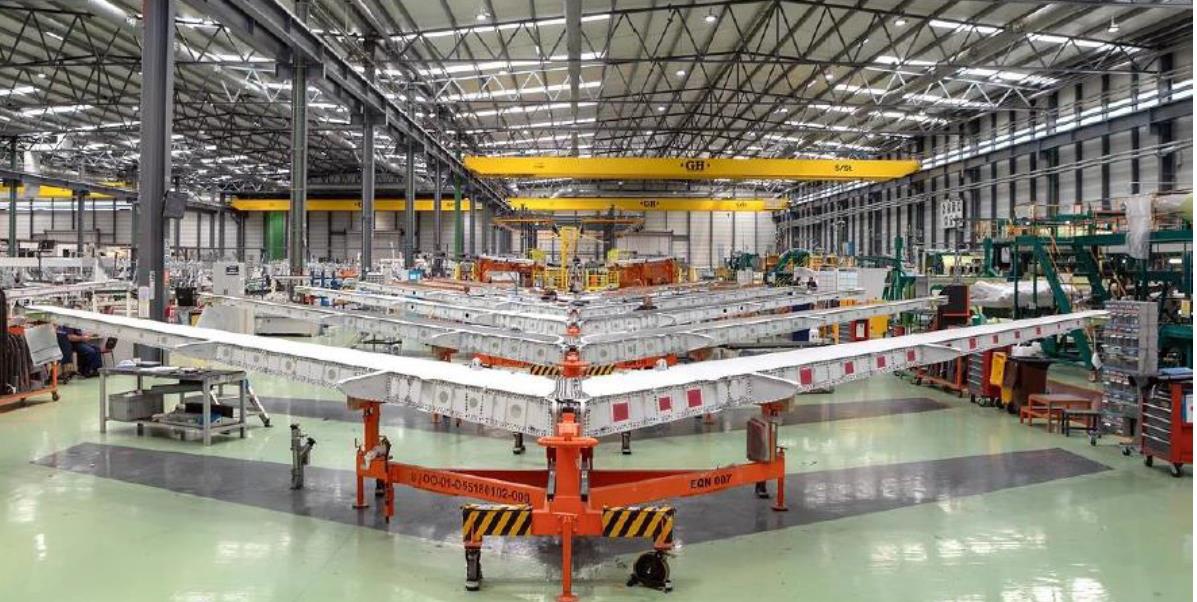
\includegraphics[height=9.25cm]{../figures/source/alestis_htp_nave.png}};
    \fill[Navy2,opacity=0.50] (9.25,0) rectangle (16,9);
  \end{scope}
  \draw[Cyan,line width=1.0pt] (9.25,0.72) -- (9.25,8.34);

  \node[anchor=west,font=\fontsize{7.2}{8.0}\selectfont\bfseries,text=Cyan] at (0.88,7.94) {LUNABOTICS \textbullet{} OFERTA T\'ECNICA Y COMERCIAL};
  \node[anchor=east] at (15.25,8.24) {
\includegraphics[width=1.34cm]{../images/logo-viu-w.png}};

  \node[anchor=west,font=\fontsize{25.5}{27.0}\selectfont\bfseries,text=white,text width=8.10cm,align=left] at (0.86,6.70) {Sistema\\AMR-FOD-Kitting};
  \node[anchor=west,font=\fontsize{12.0}{13.5}\selectfont\bfseries,text=white!82,text width=7.70cm,align=left] at (0.92,4.72) {Automatizaci\'on intralog\'istica para HTP A320 y secci\'on 19.1};
  \draw[Cyan,line width=1.15pt] (0.94,4.06) -- (4.92,4.06);

  \node[anchor=west,font=\fontsize{7.2}{8.4}\selectfont,text=white!78,text width=7.25cm,align=left] at (0.94,3.18) {Actividad 1 \textbullet{} Sistemas Rob\'oticos M\'oviles\\Profesor: Jos\'e I. I\~niguez\\Autor: Jorge Luis Mayorga Taborda\\Entrega: 26 de mayo de 2026};

  \node[anchor=west,font=\fontsize{6.6}{7.5}\selectfont\bfseries,text=Cyan] at (0.94,1.36) {TESIS};
  \node[anchor=west,font=\fontsize{8.2}{9.3}\selectfont\bfseries,text=white,text width=6.95cm,align=left] at (0.94,0.88) {Medir un piloto AMR antes de escalar la flota.};

  \fill[white,opacity=0.92,rounded corners=5pt] (9.88,1.78) rectangle (14.55,3.42);
  \draw[Amber,line width=0.55pt,rounded corners=5pt] (9.88,1.78) rectangle (14.55,3.42);
  \node[anchor=west,font=\fontsize{6.1}{6.9}\selectfont\bfseries,text=Amber] at (10.16,3.08) {CASO PILOTO};
  \node[anchor=west,font=\fontsize{12.0}{13.0}\selectfont\bfseries,text=Navy] at (10.16,2.58) {HTP A320 · 19.1};
  \node[anchor=west,font=\fontsize{6.2}{7.1}\selectfont,text=Ink,text width=3.92cm] at (10.18,2.08) {Kits, RFID/QR, registro de entregas e inspecci\'on FOD.};

  \node[anchor=west,font=\fontsize{5.4}{6.1}\selectfont,text=white!72,text width=3.82cm,align=left] at (9.88,0.94) {Foto base: Alestis HTP. Propuesta MROB-VIU 2026.};

  \webcamplaceholder
\end{scope}
\end{tikzpicture}

\speakernote{Abrir con calma. Presento la propuesta como una oferta técnica y comercial para estabilizar la logística auxiliar alrededor del HTP A320 en la sección 19.1. La idea central es medir un piloto AMR antes de escalar. En una frase: Lunabotics propone mover kits, útiles y consumibles con trazabilidad, y usar CoppeliaSim para validar la lógica de misión antes de entrar en planta.}

% 2
\startslide{Mensaje ejecutivo}{Necesidad, piloto y decisi\'on}{Violet}
  \node[anchor=west,font=\fontsize{11.0}{12.2}\selectfont\bfseries,text=Navy,text width=13.10cm] at (1.00,6.56) {El piloto mide seguridad, trazabilidad y tiempos antes de comprar una flota.};

  \foreach \x/\num/\ttl/\txt/\col in {
    1.05/{01}/{Problema}/{8--15\% del turno en log\'istica auxiliar; hip\'otesis de entrevista}/Amber,
    5.45/{02}/{Piloto}/{1 AMR omnidireccional + sensores integrados + 237 k\texteuro{}}/Teal,
    9.85/{03}/{Decisi\'on}/{escalado 1 \(\rightarrow\) 7 \(\rightarrow\) 17 condicionado a KPIs y umbral econ\'omico}/Green}{
    \fill[\col!10,rounded corners=6pt] (\x,4.05) rectangle ++(3.92,1.42);
    \draw[\col,line width=0.55pt,rounded corners=6pt] (\x,4.05) rectangle ++(3.92,1.42);
    \node[anchor=west,font=\fontsize{14.0}{15.2}\selectfont\bfseries,text=\col] at (\x+0.22,5.08) {\num};
    \node[anchor=west,font=\fontsize{7.4}{8.3}\selectfont\bfseries,text=Navy] at (\x+1.02,5.10) {\ttl};
    \node[anchor=north west,font=\fontsize{5.75}{6.55}\selectfont,text=Ink,text width=3.42cm,align=left] at (\x+0.24,4.72) {\txt};
  }

  \draw[Line,line width=0.65pt] (1.05,3.44) -- (14.32,3.44);
  \foreach \x/\ttl/\txt/\col in {
    1.05/{Log\'istica auxiliar estable}/{reduce variabilidad alrededor del HTP}/Teal,
    5.45/{Criterios m\'inimos del piloto}/{misiones, registro, disponibilidad y seguridad}/Violet,
    9.85/{CAPEX estimado sin IVA}/{237.444 \texteuro{} piloto; 1,10 M\texteuro{} expansi\'on}/Amber}{
    \node[anchor=west,font=\fontsize{6.6}{7.6}\selectfont\bfseries,text=\col] at (\x,2.88) {\ttl};
    \node[anchor=north west,font=\fontsize{5.9}{6.8}\selectfont,text=Muted,text width=3.70cm,align=left] at (\x,2.52) {\txt};
  }

  \fill[Violet!9,rounded corners=5pt] (1.05,0.88) rectangle (14.40,1.64);
  \draw[Violet!38,line width=0.45pt,rounded corners=5pt] (1.05,0.88) rectangle (14.40,1.64);
  \node[anchor=west,font=\fontsize{6.5}{7.4}\selectfont\bfseries,text=Navy,text width=12.58cm] at (1.28,1.28) {Alcance: el AMR estabiliza soporte log\'istico; fabricaci\'on, inspecci\'on certificada y decisiones de calidad quedan fuera del piloto.};
\stopslide
\speakernote{Esta slide es el mapa ejecutivo. Primero, el problema: una parte del turno se consume en logística auxiliar y hay que validarlo en planta. Segundo, el piloto: un AMR omnidireccional con RFID/QR, sensores y HMI para una zona acotada. Tercero, la decisión: la flota escala de 1 a 7 y después a 17 solo si los KPIs y el umbral económico lo justifican.}

% 3
\startslide{Lunabotics}{Integrador de rob\'otica m\'ovil industrial}{Teal}
  \begin{scope}
    \clip (0.90,1.10) rectangle (6.55,6.86);
    \node[anchor=center,opacity=0.25] at (3.68,3.98) {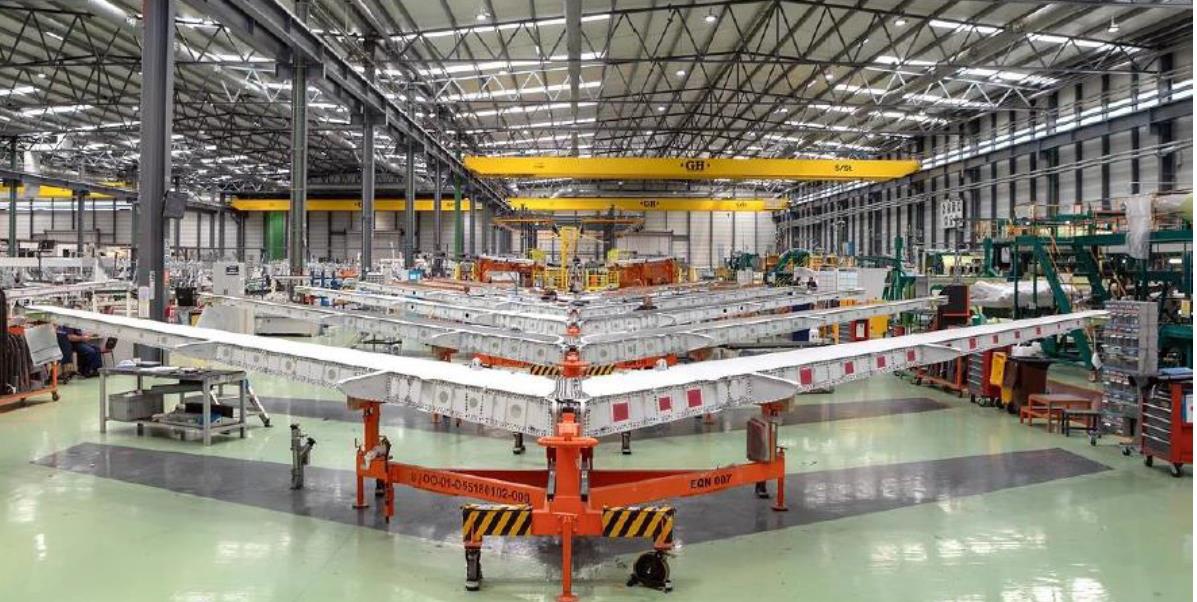
\includegraphics[height=5.9cm]{../figures/source/alestis_htp_nave.png}};
    \fill[Navy,opacity=0.72] (0.90,1.10) rectangle (6.55,6.86);
  \end{scope}
  \node[anchor=west,font=\fontsize{7.0}{8.0}\selectfont\bfseries,text=Cyan] at (1.18,6.30) {QUI\'ENES SOMOS};
  \node[anchor=west,font=\fontsize{18.5}{20.0}\selectfont\bfseries,text=white,text width=4.70cm,align=left] at (1.18,5.45) {Pilotos AMR antes de flota.};
  \node[anchor=west,font=\fontsize{7.1}{8.3}\selectfont,text=white!84,text width=4.80cm,align=left] at (1.20,3.86) {Lunabotics integra rob\'otica m\'ovil industrial para transporte, inspecci\'on y trazabilidad en planta.};

  \node[anchor=west,font=\fontsize{12.2}{13.4}\selectfont\bfseries,text=Navy] at (7.15,6.42) {Capacidades para esta oferta};
  \signal{7.28}{5.42}{An\'alisis de flujo, misiones AMR y puntos de entrega/retorno.}{Teal}
  \signal{7.28}{4.56}{Modelado en CoppeliaSim con YouBot/Omnirob como proxy holon\'omico.}{Violet}
  \signal{7.28}{3.82}{Selecci\'on industrial: plataforma, sensores, safety pack y HMI.}{Amber}
  \signal{7.28}{3.02}{Integraci\'on de RFID/QR, registro de misiones y evidencia FOD.}{Green}

  \draw[Line,line width=0.6pt] (7.12,2.22) -- (14.82,2.22);
  \foreach \x/\num/\lab/\col in {
    7.28/{ROS 2}/{Nav2, misiones y registro}/Teal,
    9.72/{ISO}/{3691-4 como marco safety}/Teal,
    12.16/{MES}/{integraci\'on limitada y trazable}/Teal}{
    \node[anchor=west,font=\fontsize{17}{18}\selectfont\bfseries,text=\col] at (\x,1.74) {\num};
    \node[anchor=west,font=\fontsize{5.9}{6.8}\selectfont,text=Muted,text width=1.75cm] at (\x,1.21) {\lab};
  }
\stopslide
\speakernote{Aquí explico por qué Lunabotics tiene sentido como proveedor ficticio de la actividad. Es una integradora pequeña, no un fabricante de aviones. Su valor está en unir ROS 2, Nav2, seguridad, HMI, datos y pruebas de planta. Esto evita vender una flota antes de tener evidencia operativa.}

% 3
\startslide{Tesis}{Estabilizar el flujo que rodea al HTP}{Teal}
  \roundbox{0.92}{1.20}{6.38}{5.80}{Cool}{Teal!35}
  \node[anchor=west,font=\fontsize{6.2}{7.0}\selectfont\bfseries,text=Teal] at (1.20,6.52) {EL OBJETIVO};
  \coordinate (gaugeC) at (4.10,3.36);
  \def\gaugeR{1.54}
  \draw[Line,line width=4.2pt,line cap=round] ($(gaugeC)+(188:\gaugeR)$) arc[start angle=188,end angle=-8,radius=\gaugeR];
  \draw[Amber,line width=4.2pt,line cap=round] ($(gaugeC)+(188:\gaugeR)$) arc[start angle=188,end angle=40,radius=\gaugeR];
  \draw[Red,line width=1.0pt,line cap=round] (gaugeC) -- ($(gaugeC)+(40:1.14)$);
  \fill[Red] (gaugeC) circle (0.075);
  \node[font=\fontsize{20}{21}\selectfont\bfseries,text=Navy] at (3.42,2.68) {40};
  \node[font=\fontsize{17}{18}\selectfont\bfseries,text=Navy] at (4.10,2.68) {\(\rightarrow\)};
  \node[font=\fontsize{20}{21}\selectfont\bfseries,text=Navy] at (4.78,2.68) {80};
  \node[font=\fontsize{6.3}{7.2}\selectfont\bfseries,text=Muted,text width=5.20cm,align=center] at (4.10,2.08) {HTP/mes: el AMR act\'ua sobre la palanca log\'istica};
  \node[anchor=west,font=\fontsize{6.0}{6.8}\selectfont\bfseries,text=Teal] at (1.28,1.62) {40 actuales};
  \node[anchor=east,font=\fontsize{6.0}{6.8}\selectfont\bfseries,text=Amber] at (6.92,1.62) {80+ objetivo 24 meses};

  \node[anchor=west,font=\fontsize{6.2}{7.0}\selectfont\bfseries,text=Muted] at (7.90,6.86) {LA SOLUCI\'ON};
  \node[anchor=north west,font=\fontsize{11.3}{12.7}\selectfont\bfseries,text=Navy,text width=7.45cm,align=left] at (7.90,6.24) {Menos esperas en estaci\'on\\con registro y FOD trazado.};
  \signal{8.04}{4.28}{AMR omnidireccional para entregar kits, \'utiles y consumibles.}{Teal}
  \signal{8.04}{3.48}{RFID/QR para cerrar cada entrega con evidencia digital.}{Violet}
  \signal{8.04}{2.68}{Rondas FOD con captura RGB-D y revisi\'on humana.}{Amber}
  \signal{8.04}{1.88}{\(\geq 98\%\) registros RFID/QR completos como objetivo del piloto.}{Green}
  \node[anchor=west,font=\fontsize{7.0}{8.2}\selectfont\bfseries,text=Ink,text width=6.20cm] at (7.90,1.14) {El robot coordina entregas y registro para liberar tiempo en la estaci\'on.};
\stopslide
\speakernote{La tesis es que el AMR actúa sobre la palanca logística del objetivo 40 a 80 HTP al mes. No afirmo que el robot duplique la producción. Lo que sí puede hacer es reducir esperas en estación, cerrar entregas con RFID/QR y generar evidencia FOD revisable. Si esa logística se estabiliza, la planta gana margen para crecer con menos variabilidad.}



% 4
\startslide{Seguridad}{L\'imites normativos antes de operar en planta}{Violet}
  \node[anchor=west,font=\fontsize{8.2}{9.3}\selectfont\bfseries,text=Navy,text width=13.25cm] at (1.02,6.48) {El AMR se trata como equipo de intralog\'istica en zona aeron\'autica: primero seguridad funcional, luego productividad.};

  \foreach \x/\ttl/\txt/\col in {
    1.05/{ISO 3691-4}/{AMR/AGV: velocidad, parada, zonas lentas y operaci\'on cerca de personas.}/Teal,
    5.05/{NAS 412 / FOD}/{El robot genera evidencia FOD revisable; la certificaci\'on queda en calidad.}/Amber,
    9.05/{AS9100 / cliente}/{Trazabilidad, cambios controlados y aceptaci\'on del proceso por planta.}/Violet,
    13.05/{CE / m\'aquinas}/{Conjunto AMR + portakits + sensores validado antes de SAT.}/Green}{
    \fill[\col!10,rounded corners=5pt] (\x,4.16) rectangle ++(2.78,1.74);
    \draw[\col,line width=0.55pt,rounded corners=5pt] (\x,4.16) rectangle ++(2.78,1.74);
    \node[anchor=west,font=\fontsize{7.3}{8.2}\selectfont\bfseries,text=\col,text width=2.35cm] at (\x+0.20,5.48) {\ttl};
    \node[anchor=north west,font=\fontsize{5.05}{5.65}\selectfont,text=Ink,text width=2.36cm] at (\x+0.20,5.08) {\txt};
  }

  \draw[Line,line width=0.65pt] (1.05,3.74) -- (14.85,3.74);
  \node[anchor=west,font=\fontsize{9.6}{10.8}\selectfont\bfseries,text=Navy] at (1.05,3.28) {Tres reglas de alcance};
  \foreach \y/\txt/\col in {
    2.72/{Seguridad funcional independiente: esc\'aner, bumper y E-stop tienen prioridad sobre Nav2.}/Red,
    2.10/{FOD preventivo: captura RGB-D + revisi\'on humana; inspecci\'on certificada por calidad.}/Amber,
    1.48/{Operaci\'on reversible: si falla el AMR, la log\'istica manual mantiene la l\'inea.}/Teal}{
    \fill[\col] (1.18,\y) circle (0.065);
    \node[anchor=west,font=\fontsize{7.0}{8.0}\selectfont\bfseries,text=Ink,text width=12.0cm] at (1.46,\y-0.02) {\txt};
  }
  \node[anchor=west,font=\fontsize{5.75}{6.55}\selectfont,text=Muted,text width=12.6cm] at (1.05,0.82) {HTP A320: estabilizador horizontal; secci\'on 19.1: zona piloto de entrega y retorno de \'utiles.};
\stopslide
\speakernote{Antes de entrar en productividad, fijo los límites de seguridad. El AMR trabaja en una nave aeronáutica, no en un almacén genérico. Por eso aparecen ISO 3691-4 para AMR/AGV, NAS 412 para FOD, AS9100 para trazabilidad y CE para el conjunto robot más portakits. La regla de defensa es simple: la seguridad funcional tiene prioridad sobre navegación y productividad.}

% 5
\startslide{Dolor operativo}{Recorridos pequeños que frenan el flujo}{Amber}
  \node[anchor=west,font=\fontsize{10.6}{11.8}\selectfont\bfseries,text=Navy,text width=6.45cm] at (0.98,6.36) {Las p\'erdidas aparecen como recorridos peque\~nos y repetidos.};
  \floorgrid{0.95}{2.02}{1.62}{Amber}
  \draw[Red,line width=1.0pt,dashed,rounded corners=8pt,->] (2.08,2.75) -- (5.55,2.75) -- (5.55,5.38) -- (2.10,5.38) -- (2.10,3.60);
  \node[anchor=west,font=\fontsize{18}{19}\selectfont\bfseries,text=Amber] at (8.72,6.22) {Esperas de planta};
  \signal{8.82}{5.18}{Operarios abandonan estaci\'on para buscar \'utiles o consumibles.}{Amber}
  \signal{8.82}{4.30}{Kits incompletos bloquean trabajo sin quedar siempre visibles como parada.}{Teal}
  \signal{8.82}{3.42}{FOD exige inspecci\'on, disciplina y evidencia revisable.}{Red}
  \signal{8.82}{2.54}{El registro se pierde si la entrega no queda ligada a una misi\'on.}{Violet}
  \node[anchor=west,font=\fontsize{6.6}{7.6}\selectfont\bfseries,text=Navy,text width=5.55cm] at (8.72,1.52) {La propuesta no sustituye al operario: reduce desplazamientos sin valor a\~nadido y documenta cada cierre.};
  \fill[Amber!12,rounded corners=4pt] (8.58,0.66) rectangle (13.66,1.08);
  \node[anchor=west,font=\fontsize{5.35}{6.1}\selectfont\bfseries,text=Amber,text width=4.82cm] at (8.72,0.87) {Supuesto a validar: log\'istica auxiliar = 8--15\% del tiempo de turno afectado.};
\stopslide
\speakernote{Aquí cuento el dolor operativo sin exagerar. Las pérdidas no siempre aparecen como grandes paradas: son salidas del operario, kits incompletos, vueltas a por útiles, FOD que obliga a revisar y registros que se cierran tarde. El rango 8--15\% es una hipótesis de entrevista que se debe medir. El piloto busca convertir ese dolor difuso en datos.}

% 6
\startslide{Contexto}{Flujo auxiliar en HTP A320 y secci\'on 19.1}{Cyan}
  % Slide 04: integrated context map for HTP A320 / section 19.1.

\fill[Cyan!8,rounded corners=10pt] (0.92,1.12) rectangle (15.08,6.92);
\draw[Cyan!35,rounded corners=10pt,line width=0.4pt] (0.92,1.12) rectangle (15.08,6.92);

\node[anchor=west,font=\fontsize{5.8}{6.6}\selectfont\bfseries,text=Cyan] at (1.26,6.54) {CONTEXTO DE PLANTA};
\node[anchor=west,font=\fontsize{16.2}{17.5}\selectfont\bfseries,text=Navy,text width=5.9cm,align=left] at (1.26,5.96) {Estructura grande;\\soporte logístico fino.};
\node[anchor=west,font=\fontsize{7.0}{8.2}\selectfont,text=Muted,text width=5.6cm,align=left] at (1.30,4.82) {El AMR no toca montaje certificado: estabiliza entregas, retorno de útiles, FOD y trazabilidad alrededor de la estaci\'on.};

\begin{scope}[shift={(1.18,2.75)},scale=1.42]
  \draw[Navy,line width=1.15pt] (0,0) .. controls (1.35,0.32) and (3.75,0.24) .. (5.25,0.02);
  \draw[Navy,line width=1.15pt] (0,-0.62) .. controls (1.35,-0.92) and (3.75,-0.84) .. (5.25,-0.63);
  \draw[Navy,line width=0.75pt] (5.25,0.02) -- (5.25,-0.63);
  \fill[Teal!72] (2.02,0.04) -- (1.02,0.68) -- (2.56,0.34) -- cycle;
  \fill[Teal!72] (2.02,-0.64) -- (1.02,-1.28) -- (2.56,-0.94) -- cycle;
  \fill[Amber!82] (3.36,0.20) rectangle (4.03,-0.82);
  \node[font=\fontsize{5.2}{5.8}\selectfont\bfseries,text=white] at (3.70,-0.30) {19.1};
  \node[anchor=west,font=\fontsize{5.6}{6.2}\selectfont\bfseries,text=Teal] at (0.88,0.97) {HTP};
\end{scope}

\draw[Line,line width=0.6pt] (7.40,1.56) -- (7.40,6.46);

\node[anchor=west,font=\fontsize{5.8}{6.6}\selectfont\bfseries,text=Cyan] at (7.86,6.54) {FLUJO QUE SE AUTOMATIZA};
\node[anchor=west,font=\fontsize{11.2}{12.4}\selectfont\bfseries,text=Ink,text width=7.15cm,align=left] at (7.86,5.92) {Kit \(\rightarrow\) entrega \(\rightarrow\) registro \(\rightarrow\) retorno};

\foreach \x/\lab/\sub/\col in {
  8.05/Kit validado/RFID--QR/Teal,
  10.72/Estaci\'on HTP/entrega trazada/Amber,
  13.38/Retorno + FOD/evidencia digital/Green} {
  \fill[\col!16,rounded corners=5pt] (\x,3.24) rectangle ++(1.78,1.02);
  \draw[\col,line width=0.5pt,rounded corners=5pt] (\x,3.24) rectangle ++(1.78,1.02);
  \node[anchor=center,font=\fontsize{6.5}{7.4}\selectfont\bfseries,text=Ink,align=center,text width=1.55cm] at (\x+0.89,3.91) {\lab};
  \node[anchor=center,font=\fontsize{5.2}{6.0}\selectfont,text=Muted,align=center,text width=1.55cm] at (\x+0.89,3.49) {\sub};
}
\draw[Cyan,arrow,line width=0.8pt] (9.95,3.75) -- (10.55,3.75);
\draw[Cyan,arrow,line width=0.8pt] (12.62,3.75) -- (13.20,3.75);

\node[anchor=west,font=\fontsize{7.4}{8.6}\selectfont\bfseries,text=Navy,text width=6.4cm,align=left] at (7.88,2.35) {Lectura clave para la propuesta};
\node[anchor=west,font=\fontsize{6.6}{7.7}\selectfont,text=Muted,text width=6.5cm,align=left] at (7.88,1.78) {La secci\'on 19.1 concentra dependencia de kits, herramientas, documentaci\'on y disciplina FOD. Ah\'i el AMR reduce esperas y deja trazas, sin fabricar el HTP.};

\stopslide
\speakernote{Esta diapositiva aterriza el contexto. El HTP es grande y el trabajo de alrededor es delicado: kits, útiles, documentación y disciplina FOD. La parte automatizable es muy concreta: validar kit, entregar en punto trazado, cerrar registro y volver con evidencia FOD. Las distancias son estimadas para el levantamiento de semana 1, no medidas definitivas.}

% 7
\startslide{Alcance}{D\'onde entra el AMR y d\'onde no entra}{Cyan}
  \node[anchor=west,font=\fontsize{6.4}{7.2}\selectfont\bfseries,text=Muted] at (0.98,6.46) {MAPA OPERATIVO SIMPLIFICADO · TIEMPOS HIP\'OTESIS S1};
  \fill[Panel,rounded corners=6pt] (1.00,1.56) rectangle (14.70,5.92);
  \draw[Line,line width=0.5pt,rounded corners=6pt] (1.00,1.56) rectangle (14.70,5.92);
  \foreach \x/\ttl/\sub/\col in {
    1.56/{Base log\'istica}/{\(\sim\)2 min carga + lectura}/Teal,
    4.60/{Pasillo seguro}/{\(\sim\)3 min ruta limitada}/Cyan,
    7.64/{Estaci\'on HTP 19.1}/{\(\sim\)1 min entrega + confirmaci\'on}/Amber,
    10.68/{Retorno / FOD}/{\(\sim\)4--6 min retorno y evidencia}/Green}{
    \fill[\col!12,rounded corners=5pt] (\x,3.08) rectangle ++(2.20,1.42);
    \draw[\col,line width=0.55pt,rounded corners=5pt] (\x,3.08) rectangle ++(2.20,1.42);
    \node[anchor=north,font=\fontsize{7.0}{7.8}\selectfont\bfseries,text=\col,align=center,text width=1.90cm] at (\x+1.10,4.17) {\ttl};
    \node[anchor=north,font=\fontsize{5.3}{6.0}\selectfont,text=Ink,align=center,text width=1.84cm] at (\x+1.10,3.58) {\sub};
  }
  \foreach \x in {3.84,6.88,9.92}{\draw[Teal,arrow,line width=0.85pt] (\x,3.78) -- (\x+0.52,3.78);}
  \roboticon{5.70}{2.26}{0.55}
  \node[anchor=west,font=\fontsize{6.4}{7.3}\selectfont\bfseries,text=Teal] at (6.48,2.28) {El robot opera en pasillos y puntos auxiliares alrededor de la estaci\'on.};
  \fill[Red!6,rounded corners=4pt] (1.08,0.82) rectangle (14.25,1.25);
  \node[anchor=west,font=\fontsize{5.85}{6.6}\selectfont\bfseries,text=Red,text width=12.75cm] at (1.28,1.04) {Fuera de alcance: montaje, mecanizado y manipulaci\'on directa del HTP. Validaci\'on humana para entrega, evento FOD y cierre con incidencia.};
\stopslide
\speakernote{Esta slide protege el alcance. El robot no entra sobre la pieza ni decide calidad. Opera en pasillos y puntos auxiliares. Los tiempos son hipótesis iniciales para dimensionar el ciclo: carga, ruta, entrega y retorno. Las decisiones sensibles, como aceptar una entrega con incidencia o revisar FOD, quedan en manos humanas.}

% 8
\startslide{Entrevista}{Hallazgos convertidos en requisitos}{Violet}
  % Slide 05: interview findings with a cleaner visual hierarchy.

\fill[Violet!8,rounded corners=8pt] (0.88,1.18) rectangle (4.55,6.78);
\draw[Violet!38,rounded corners=8pt,line width=0.45pt] (0.88,1.18) rectangle (4.55,6.78);
\node[anchor=north west,font=\fontsize{5.9}{6.6}\selectfont\bfseries,text=Violet] at (1.12,6.52) {ACTA T\'ECNICA};
\node[anchor=north west,font=\fontsize{10.4}{11.6}\selectfont\bfseries,text=Navy] at (1.12,6.06) {Carlos P\'erez};
\node[anchor=north west,font=\fontsize{6.1}{7.0}\selectfont,text=Muted,text width=2.98cm] at (1.12,5.62) {+10 a\~nos en Alestis Puerto Real. Entrevista guiada con el prompt oficial.};

\node[anchor=north west,font=\fontsize{12.0}{13.0}\selectfont\bfseries,text=Navy,text width=3.02cm,align=left] at (1.12,4.54) {No pong\'ais el robot a fabricar. Ponedlo a quitar paseos.};
\draw[Violet,line width=0.9pt] (1.14,2.70) -- (3.90,2.70);
\node[anchor=north west,font=\fontsize{6.35}{7.35}\selectfont,text=Muted,text width=3.05cm,align=left] at (1.12,2.34) {La entrevista se traduce en cuatro decisiones de dise\~no y en KPIs del piloto.};

\node[anchor=west,font=\fontsize{6.0}{6.8}\selectfont\bfseries,text=Muted] at (5.20,6.56) {DE HALLAZGO A DECISI\'ON};

\foreach \y/\num/\col/\ttl/\txt in {
  5.65/01/Violet/{Alcance correcto}/{Log\'istica auxiliar: kits, herramientas, retorno y registro.},
  4.46/02/Teal/{Pasillos cambiantes}/{Base omnidireccional con SLAM y gestor de misiones.},
  3.27/03/Amber/{FOD con evidencia}/{Ronda RGB-D, evento trazado y revisi\'on humana.},
  2.08/04/Green/{Escalado con datos}/{Pasar de 1 a 7 robots solo si los KPIs lo justifican.}
}{
  \fill[\col!12,rounded corners=5pt] (5.18,\y-0.42) rectangle (14.95,\y+0.45);
  \draw[\col,line width=0.45pt,rounded corners=5pt] (5.18,\y-0.42) rectangle (14.95,\y+0.45);
  \fill[\col] (5.58,\y+0.02) circle (0.16);
  \node[font=\fontsize{5.3}{5.9}\selectfont\bfseries,text=white] at (5.58,\y+0.02) {\num};
  \node[anchor=west,font=\fontsize{7.4}{8.3}\selectfont\bfseries,text=Ink,text width=2.75cm,align=left] at (5.92,\y+0.13) {\ttl};
  \node[anchor=west,font=\fontsize{6.45}{7.35}\selectfont,text=Ink,text width=6.00cm,align=left] at (8.38,\y+0.13) {\txt};
}

\node[anchor=west,font=\fontsize{5.9}{6.8}\selectfont\bfseries,text=Red] at (5.22,1.20) {Evidencia pendiente de entrega: capturas reales de ChatGPT en el anexo.};

\stopslide
\speakernote{La entrevista simulada con Carlos Pérez traduce el problema de planta a requisitos. El mensaje que uso es: menos vueltas y cada entrega registrada. De ahí salen cuatro decisiones: limitar el alcance a logística auxiliar, usar AMR con SLAM para pasillos cambiantes, registrar FOD con evidencia y escalar solo con datos. Las capturas están en el anexo del informe.}

% 6
\startslide{Requisitos}{Criterios de aceptación conectados con el temario}{Teal}
  \foreach \x/\val/\lab/\col in {
    1.25/\(\geq 95\%\)/misiones completadas en piloto/Teal,
    4.95/\(\geq 98\%\)/registro completo por misi\'on/Green,
    8.65/\(\geq 90\%\)/disponibilidad AMR en turno/Cyan,
    12.35/{0}/{contactos no previstos\\0 incidentes con da\~no}/Red}{
    \node[anchor=west,font=\fontsize{19}{20}\selectfont\bfseries,text=\col] at (\x,6.05) {\val};
    \node[anchor=west,font=\fontsize{7.2}{8.4}\selectfont,text=Ink,text width=2.7cm] at (\x,5.32) {\lab};
    \draw[\col,line width=1.4pt] (\x,5.00) -- (\x+2.60,5.00);
  }
  \draw[Line,line width=0.6pt] (1.00,3.80) -- (14.85,3.80);
  \node[anchor=west,font=\fontsize{9.2}{10.3}\selectfont\bfseries,text=Navy] at (1.05,3.30) {Traducción técnica desde el curso};
  \foreach \x/\ttl/\txt/\col in {
    1.05/Locomoción/base mecanum-sueca con maniobra lateral/Green,
    4.75/Percepción/{LiDAR \textbullet{} RGB-D \textbullet{} RFID--QR; safety independiente}/Teal,
    8.45/Navegación/{SLAM + global A*--Dijkstra + local TEB}/Cyan,
    12.15/Control/{motores con encoders, límites de velocidad por zona y E-stop}/Red}{
    \node[anchor=west,font=\fontsize{7.0}{8.0}\selectfont\bfseries,text=\col] at (\x,2.78) {\ttl};
    \node[anchor=north west,font=\fontsize{6.0}{7.0}\selectfont,text=Ink,text width=3.1cm,align=left] at (\x,2.36) {\txt};
  }
  \fill[Teal!8,rounded corners=4pt] (1.00,0.86) rectangle (14.34,1.46);
  \draw[Teal!35,line width=0.35pt,rounded corners=4pt] (1.00,0.86) rectangle (14.34,1.46);
  \node[anchor=west,font=\fontsize{5.75}{6.55}\selectfont\bfseries,text=Navy,text width=12.60cm] at (1.22,1.18) {Fuente de medición: log de misiones, RFID/QR, estado AMR, eventos safety y revisión FOD en HMI/dashboard.};
\stopslide
\speakernote{Aquí conecto la propuesta con criterios medibles. Para aprobar el piloto pido al menos 95\% de misiones completadas, 98\% de registro completo, 90\% de disponibilidad y cero contactos no previstos. También indico cómo se mide: logs de misión, RFID/QR, estado AMR, eventos safety y revisión FOD en HMI o dashboard.}

% 7
\startslide{Alternativas}{Matriz de decisión con criterios ponderados}{Cyan}
  \node[anchor=west,font=\fontsize{7.0}{8.0}\selectfont\bfseries,text=Muted] at (0.95,6.28) {PUNTUACIÓN PONDERADA SOBRE 5};
  \node[anchor=west,font=\fontsize{25}{26}\selectfont\bfseries,text=Green] at (0.95,5.58) {4,20};
  \node[anchor=west,font=\fontsize{9.1}{10.2}\selectfont\bfseries,text=Navy,text width=5.15cm,align=left] at (3.28,5.73) {AMR omnidireccional\\RB-KAIROS/AGILOX-class};
  \node[anchor=west,font=\fontsize{6.2}{7.1}\selectfont,text=Muted,text width=6.75cm] at (0.98,4.90) {Se prioriza maniobra en estación y madurez de validación, aunque no sea la opción más barata.};

  \foreach \y/\name/\score/\w/\col in {
    4.18/{AMR omnidireccional}/{4,20}/4.49/Green,
    3.54/{AMR diferencial MiR/Omron}/{3,90}/4.17/Teal,
    2.90/{AGV}/{3,15}/3.37/Amber,
    2.26/{Robot con patas}/{1,85}/1.98/Violet,
    1.62/{Dron}/{1,80}/1.93/Red,
    0.98/{Orugas}/{1,45}/1.55/Muted} {
    \node[anchor=west,font=\fontsize{6.4}{7.3}\selectfont\bfseries,text=Ink] at (0.98,\y+0.11) {\name};
    \fill[\col!18] (4.40,\y) rectangle ++(4.85,0.23);
    \fill[\col] (4.40,\y) rectangle ++(\w,0.23);
    \node[anchor=west,font=\fontsize{6.2}{7.0}\selectfont\bfseries,text=\col] at (9.45,\y+0.02) {\score};
  }

  \draw[Line,line width=0.6pt] (10.55,1.04) -- (10.55,6.20);
  \node[anchor=west,font=\fontsize{9.5}{10.7}\selectfont\bfseries,text=Navy] at (11.05,6.02) {criterios con peso};
  \foreach \y/\txt/\col in {
    5.40/{25\% maniobra en estación.}/Green,
    4.76/{20\% seguridad con operarios.}/Red,
    4.12/{15\% registro e integración.}/Violet,
    3.48/{15\% madurez comercial.}/Teal,
    2.84/{15\% coste/riesgo de integración.}/Amber,
    2.20/{10\% madurez en simulaci\'on.}/Cyan}{
    \fill[\col] (11.12,\y) circle (0.075);
    \node[anchor=west,font=\fontsize{7.0}{8.1}\selectfont,text=Ink,align=left,text width=3.78cm] at (11.39,\y-0.02) {\txt};
  }
  \node[anchor=west,font=\fontsize{5.4}{6.2}\selectfont\bfseries,text=Muted,text width=8.80cm] at (0.98,0.54) {El omni gana por maniobra en estación, el criterio de mayor peso. La diferencia frente al diferencial se defiende por espacio operativo.};
  \node[anchor=west,font=\fontsize{5.25}{6.0}\selectfont\bfseries,text=Muted,text width=3.85cm] at (11.05,1.42) {Criterio acad\'emico convertido a validaci\'on industrial.};
\stopslide
\speakernote{La matriz explica por qué gana el AMR omnidireccional. La diferencia frente al diferencial no es enorme, pero aparece en el criterio que más pesa: maniobra junto a estaciones. Un AGV es predecible, pero pierde flexibilidad en una planta existente. El dron, patas y orugas se descartan por seguridad, carga, mantenimiento o aceptación.}

% 8
\startslide{Robot}{Modelo elegido y opciones reales de compra}{Green}
  \roundbox{0.92}{1.18}{7.42}{5.72}{Panel}{Green!35}
  \node[anchor=center] at (4.55,4.20) {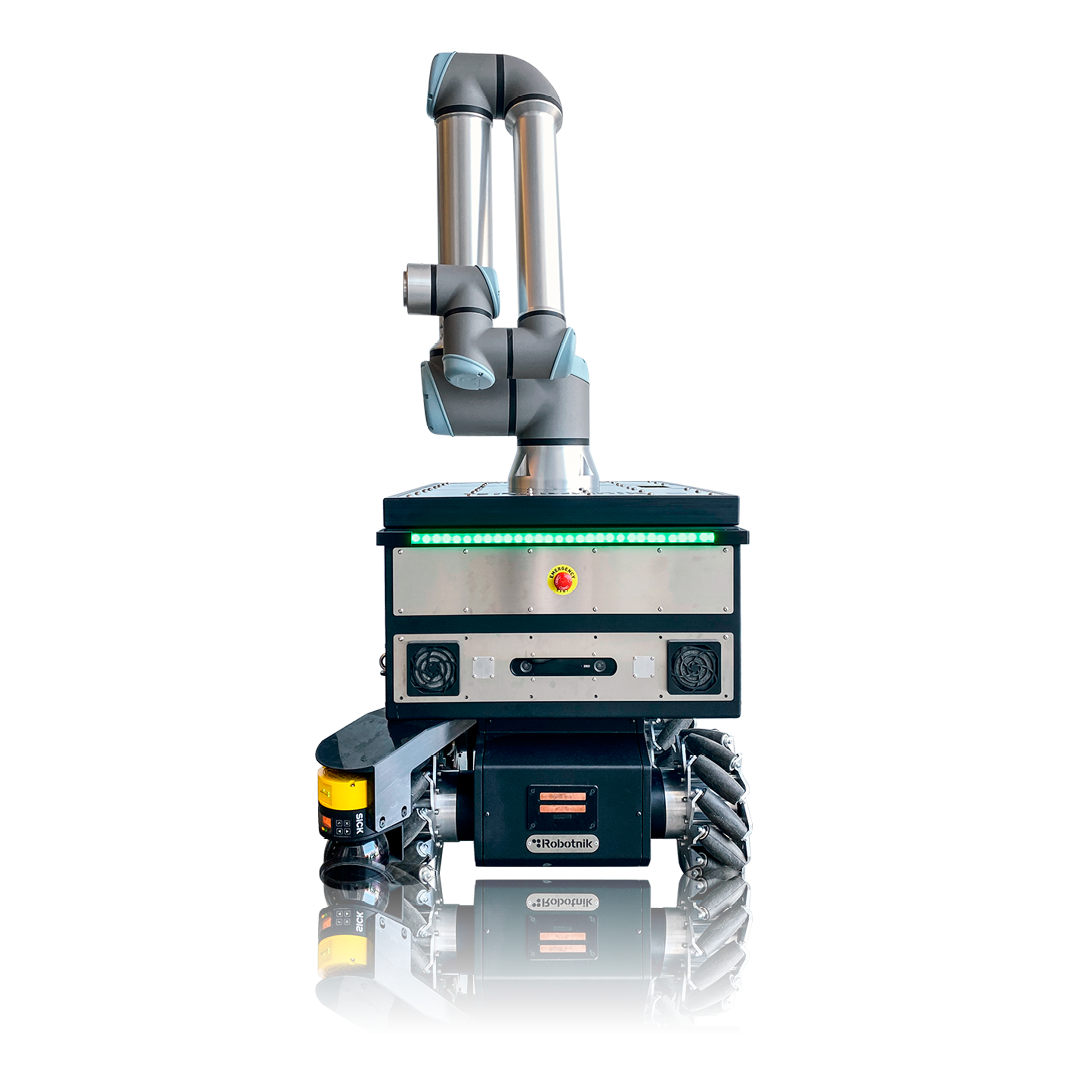
\includegraphics[width=5.25cm,trim=0 0 0 385,clip]{../figures/source/robotnik_rb_kairos.png}};
  \node[anchor=west,font=\fontsize{7.0}{8.0}\selectfont\bfseries,text=Green] at (1.20,6.48) {REFERENCIA INDUSTRIAL};
  \fill[Amber!16,rounded corners=4pt] (1.20,1.50) rectangle (7.92,2.10);
  \draw[Amber,line width=0.55pt,rounded corners=4pt] (1.20,1.50) rectangle (7.92,2.10);
  \node[anchor=west,font=\fontsize{5.95}{6.65}\selectfont\bfseries,text=Navy,text width=6.25cm] at (1.38,1.86) {Solo base m\'ovil + portakits};
  \node[anchor=west,font=\fontsize{5.15}{5.85}\selectfont\bfseries,text=Red,text width=6.25cm] at (1.38,1.61) {Sin brazo manipulador ni manipulaci\'on directa del HTP.};

  \foreach \x/\y/\w/\ttl/\txt/\col in {
    1.18/5.36/2.38/{Plataforma}/{holon\'omica, 250 kg, 1,5 m/s}/Green,
    1.18/2.28/2.42/{Trazabilidad}/{RFID + QR por kit}/Violet,
    5.82/5.36/2.18/{M\'odulo}/{portakits y bandejas}/Amber,
    5.82/2.28/2.18/{Inspecci\'on}/{RGB-D para FOD}/Teal}{
    \fill[\col!11,rounded corners=4pt] (\x,\y) rectangle ++(\w,0.66);
    \draw[\col,line width=0.45pt,rounded corners=4pt] (\x,\y) rectangle ++(\w,0.66);
    \node[anchor=west,font=\fontsize{5.9}{6.6}\selectfont\bfseries,text=\col] at (\x+0.12,\y+0.44) {\ttl};
    \node[anchor=west,font=\fontsize{5.1}{5.8}\selectfont,text=Ink,text width=\w cm] at (\x+0.12,\y+0.18) {\txt};
  }
  \draw[Green,line width=0.45pt] (3.56,5.68) -- (4.20,4.86);
  \draw[Violet,line width=0.45pt] (3.62,2.58) -- (4.25,3.28);
  \draw[Amber,line width=0.45pt] (5.78,5.68) -- (5.08,4.90);
  \draw[Teal,line width=0.45pt] (5.78,2.58) -- (5.08,3.15);

  \node[anchor=north west,font=\fontsize{11.2}{12.3}\selectfont\bfseries,text=Navy,text width=5.45cm] at (9.05,6.56) {Opciones industriales comparadas};
  \signal{9.18}{5.18}{Selecci\'on: RB-KAIROS-class; base holon\'omica, ROS 2 y carga \(\sim\)250 kg.}{Green}
  \signal{9.18}{4.28}{Alternativa madura: AGILOX ODM para intralog\'istica 300 kg.}{Teal}
  \signal{9.18}{3.38}{Descartado: KUKA omniMove; sobredimensionado para HTP 19.1.}{Red}
  \node[anchor=north west,font=\fontsize{6.35}{7.25}\selectfont\bfseries,text=Cyan,text width=5.35cm] at (9.18,2.34) {Simulaci\'on: YouBot/Omnirob como proxy mecanum equivalente en CoppeliaSim.};
  \node[anchor=north west,font=\fontsize{6.05}{6.85}\selectfont,text=Muted,text width=4.95cm] at (9.18,1.64) {Compra real: safety pack, portakits, registro, FAT/SAT y validaci\'on CE del conjunto.};
\stopslide
\speakernote{La selección industrial es una plataforma tipo RB-KAIROS o AGILOX ODM, pero la simulación docente usa YouBot u Omnirob como proxy mecanum. Esto es importante: compra y simulación no son lo mismo. En el piloto real no hay brazo manipulador ni manipulación del HTP; se usa base móvil con módulo portakits, sensores y seguridad.}

% 11
\startslide{Dimensionamiento}{El n\'umero de robots sale de misiones y ciclo}{Green}
  \node[anchor=west,font=\fontsize{8.2}{9.4}\selectfont\bfseries,text=Navy,text width=12.60cm] at (1.00,6.48) {Para el objetivo de 80 HTP/mes, el c\'alculo evita elegir 7 robots como n\'umero arbitrario.};

  \foreach \x/\val/\lab/\sub/\col in {
    1.05/{80}/{HTP/mes}/{20 d\'ias productivos \(\rightarrow\) 4 HTP/d\'ia}/Teal,
    4.42/{41}/{misiones/HTP}/{kit, reposici\'on, retorno y FOD}/Amber,
    7.79/{164}/{misiones/d\'ia}/{base antes de margen}/Violet,
    11.16/{15\%}/{margen}/{\(\approx\) 189 misiones/d\'ia}/Green}{
    \fill[\col!10,rounded corners=6pt] (\x,4.42) rectangle ++(2.78,1.52);
    \draw[\col,line width=0.55pt,rounded corners=6pt] (\x,4.42) rectangle ++(2.78,1.52);
    \node[anchor=west,font=\fontsize{18.2}{19.2}\selectfont\bfseries,text=\col] at (\x+0.22,5.42) {\val};
    \node[anchor=west,font=\fontsize{6.35}{7.15}\selectfont\bfseries,text=Navy,text width=2.34cm] at (\x+0.25,5.02) {\lab};
    \node[anchor=west,font=\fontsize{5.25}{6.00}\selectfont,text=Muted,text width=2.24cm] at (\x+0.25,4.67) {\sub};
  }
  \foreach \x in {3.98,7.35,10.72}{\draw[Green,arrow,line width=0.8pt] (\x,5.18) -- (\x+0.28,5.18);}

  \roundbox{1.05}{2.02}{4.10}{1.54}{Green!8}{Green!42}
  \node[anchor=west,font=\fontsize{5.8}{6.6}\selectfont\bfseries,text=Green] at (1.26,3.18) {DESGLOSE 41 MISIONES/HTP};
  \node[anchor=west,font=\fontsize{6.45}{7.35}\selectfont\bfseries,text=Navy,text width=3.68cm] at (1.26,2.74) {15 kits + 10 reposiciones + 8 retornos + 5 FOD + 3 consumibles.};

  \roundbox{5.72}{2.02}{4.10}{1.54}{Amber!8}{Amber!42}
  \node[anchor=west,font=\fontsize{5.8}{6.6}\selectfont\bfseries,text=Amber] at (5.94,3.18) {CAPACIDAD POR ROBOT};
  \node[anchor=west,font=\fontsize{5.65}{6.45}\selectfont\bfseries,text=Navy,text width=3.68cm] at (5.94,2.78) {\(8\mathrm{h}\times60\times0{,}70/12 \approx 28\) misiones/d\'ia. 12 min y 70\% son hip\'otesis conservadoras a validar.};

  \roundbox{10.38}{2.02}{4.10}{1.54}{Violet!8}{Violet!42}
  \node[anchor=west,font=\fontsize{5.8}{6.6}\selectfont\bfseries,text=Violet] at (10.60,3.18) {C\'ALCULO DE EXPANSI\'ON};
  \node[anchor=west,font=\fontsize{6.45}{7.35}\selectfont\bfseries,text=Navy,text width=3.62cm] at (10.60,2.74) {189 / 28 = 6,75 \(\rightarrow\) 7 robots para l\'inea HTP con margen.};

  \draw[Line,line width=0.65pt] (1.05,1.48) -- (14.58,1.48);
  \node[anchor=west,font=\fontsize{6.25}{7.15}\selectfont\bfseries,text=Navy,text width=11.80cm] at (1.05,1.06) {17 robots: escenario aspiracional condicionado a doble turno, zonas adicionales o reserva de mantenimiento; no se compromete sin datos.};
\stopslide
\speakernote{Esta es la defensa del número de robots. Para 80 HTP al mes uso 20 días productivos, por tanto 4 HTP al día. Con 41 misiones por HTP salen 164 misiones diarias, y con 15\% de margen unas 189. Un robot cubre unas 28 misiones por turno con 12 minutos por misión y 70\% de disponibilidad, ambos como hipótesis conservadoras a validar. Por eso 189 entre 28 da 7 robots.}

% 12
\startslide{Arquitectura}{Control por capas: navegar, actuar y dejar evidencia}{Teal}
  \node[anchor=west,font=\fontsize{6.2}{7.0}\selectfont\bfseries,text=Teal] at (1.00,6.54) {ARQUITECTURA DEL PILOTO: SENSOR \(\rightarrow\) DECISI\'ON \(\rightarrow\) EVIDENCIA};

  \node[anchor=west,font=\fontsize{6.1}{6.9}\selectfont\bfseries,text=Muted] at (1.05,5.92) {CADENA DE CONTROL};
  \foreach \x/\ttl/\sub/\col in {
    1.10/{Percepci\'on}/{LiDAR, RGB-D, RFID/QR}/Teal,
    4.18/{Localizaci\'on}/{SLAM, IMU y encoders}/Cyan,
    7.26/{Planificaci\'on}/{global A*/Dijkstra; local TEB}/Amber,
    10.34/{Control}/{\(v_x\), \(v_y\), \(\omega\) \(\rightarrow\) ruedas mecanum}/Green}{
    \fill[\col!10,rounded corners=6pt] (\x,4.56) rectangle ++(2.28,1.10);
    \draw[\col,line width=0.55pt,rounded corners=6pt] (\x,4.56) rectangle ++(2.28,1.10);
    \node[anchor=west,font=\fontsize{7.0}{7.8}\selectfont\bfseries,text=\col] at (\x+0.20,5.28) {\ttl};
    \node[anchor=west,font=\fontsize{5.35}{6.05}\selectfont,text=Ink,text width=1.82cm] at (\x+0.20,4.86) {\sub};
  }
  \foreach \x in {3.52,6.60,9.68}{\draw[Muted,arrow,line width=0.70pt] (\x,5.11) -- (\x+0.42,5.11);}

  \node[anchor=west,font=\fontsize{6.1}{6.9}\selectfont\bfseries,text=Muted] at (1.05,3.76) {CAPAS TRANSVERSALES};
  \foreach \y/\ttl/\txt/\col in {
    3.24/{Supervisi\'on}/{WMS, dashboard y decisi\'on de escalado}/Teal,
    2.72/{Proceso}/{kit, entrega, retorno y ronda FOD}/Cyan,
    2.20/{Integraci\'on}/{HMI, BD, MES/ERP y registro}/Amber,
    1.68/{Seguridad funcional}/{esc\'aner, bumper y E-stop}/Red}{
    \fill[\col!10,rounded corners=3pt] (1.05,\y-0.17) rectangle (6.58,\y+0.19);
    \draw[\col,line width=0.35pt,rounded corners=3pt] (1.05,\y-0.17) rectangle (6.58,\y+0.19);
    \node[anchor=west,font=\fontsize{5.55}{6.2}\selectfont\bfseries,text=\col,text width=1.82cm] at (1.24,\y+0.01) {\ttl};
    \node[anchor=west,font=\fontsize{4.88}{5.45}\selectfont,text=Ink,text width=3.03cm,align=left] at (3.18,\y+0.01) {\txt};
  }

  \fill[Red!8,rounded corners=5pt] (7.02,2.82) rectangle (13.20,3.62);
  \draw[Red,line width=0.50pt,rounded corners=5pt] (7.02,2.82) rectangle (13.20,3.62);
  \node[anchor=west,font=\fontsize{6.35}{7.1}\selectfont\bfseries,text=Red] at (7.28,3.38) {Regla de seguridad};
  \node[anchor=west,font=\fontsize{5.65}{6.35}\selectfont,text=Ink,text width=5.30cm] at (7.28,3.06) {Prioridad sobre navegaci\'on: intrusi\'on, contacto o parada manual detienen la misi\'on.};

  \fill[Teal!9,rounded corners=5pt] (7.02,1.62) rectangle (13.20,2.48);
  \draw[Teal,line width=0.50pt,rounded corners=5pt] (7.02,1.62) rectangle (13.20,2.48);
  \node[anchor=west,font=\fontsize{6.35}{7.1}\selectfont\bfseries,text=Teal] at (7.28,2.24) {Registro de misi\'on};
  \node[anchor=west,font=\fontsize{5.55}{6.25}\selectfont,text=Ink,text width=5.35cm] at (7.28,1.90) {robot\_id, kit\_id, origen, destino, ruta, RFID, QR, timestamps y evento\_FOD.};
\stopslide
\speakernote{La arquitectura se lee de izquierda a derecha: percibir, localizar, planificar, controlar e integrar. Lo importante es que no es solo mover el robot. Cada misión deja rastro: robot, kit, origen, destino, ruta, RFID, QR, tiempos y evento FOD. La capa de seguridad queda por encima de la navegación: si hay escáner, bumper o E-stop, la misión se detiene.}

% 10
\startslide{Operaci\'on}{Un ciclo cerrado: pedir, mover, confirmar, registrar}{Cyan}
  \node[anchor=west,font=\fontsize{6.2}{7.0}\selectfont\bfseries,text=Cyan] at (1.00,6.60) {MISI\'ON DE KITTING: FLUJO OPERATIVO};

  \foreach \x/\w/\ttl/\txt/\col in {
    1.02/3.72/{ANTES}/{preparar y validar material}/Teal,
    4.92/4.20/{DURANTE}/{mover, navegar y entregar}/Amber,
    9.30/3.70/{DESPU\'ES}/{registro FOD y retorno}/Violet}{
    \fill[\col!9,rounded corners=5pt] (\x,5.32) rectangle ++(\w,0.82);
    \draw[\col,line width=0.45pt,rounded corners=5pt] (\x,5.32) rectangle ++(\w,0.82);
    \node[anchor=west,font=\fontsize{6.2}{6.9}\selectfont\bfseries,text=\col] at (\x+0.18,5.88) {\ttl};
    \node[anchor=west,font=\fontsize{5.35}{6.05}\selectfont,text=Ink] at (\x+0.18,5.56) {\txt};
  }

  \draw[Line,line width=1.0pt] (1.46,4.44) -- (12.20,4.44);
  \foreach \x/\n/\ttl/\txt/\col in {
    1.65/1/{Planificar}/{HMI/MES lanza orden de entrega}/Teal,
    3.65/2/{Validar kit}/{carga, RFID/QR y destino}/Green,
    5.65/3/{Navegar}/{ruta SLAM y obst\'aculos}/Cyan,
    7.65/4/{Entregar}/{aproximaci\'on lateral y confirmaci\'on}/Amber,
    9.65/5/{Registro FOD}/{captura RGB-D y evento}/Red,
    11.65/6/{Retornar}/{\'utiles y cierre en BD}/Violet}{
    \fill[\col] (\x,4.44) circle (0.18);
    \node[font=\fontsize{5.1}{5.6}\selectfont\bfseries,text=white] at (\x,4.44) {\n};
    \draw[\col,line width=0.5pt] (\x,4.26) -- (\x,3.94);
    \fill[\col!9,rounded corners=5pt] (\x-0.82,2.50) rectangle ++(1.64,1.44);
    \draw[\col,line width=0.45pt,rounded corners=5pt] (\x-0.82,2.50) rectangle ++(1.64,1.44);
    \node[anchor=north,font=\fontsize{6.15}{6.85}\selectfont\bfseries,text=\col,align=center,text width=1.40cm] at (\x,3.68) {\ttl};
    \node[anchor=north,font=\fontsize{4.95}{5.55}\selectfont,text=Ink,align=center,text width=1.34cm] at (\x,3.17) {\txt};
  }

  \fill[Cyan!12,rounded corners=5pt] (1.05,1.24) rectangle (12.74,1.92);
  \draw[Cyan,line width=0.45pt,rounded corners=5pt] (1.05,1.24) rectangle (12.74,1.92);
  \node[font=\fontsize{8.2}{9.0}\selectfont\bfseries,text=Navy] at (6.90,1.61) {La misi\'on ya guarda entrega, ruta, excepci\'on y FOD.};
  \node[anchor=west,font=\fontsize{5.85}{6.65}\selectfont,text=Ink,text width=11.20cm] at (1.10,0.94) {Confirmaci\'on m\'inima en recepci\'on, sin abandonar el puesto ni a\~nadir una tarea administrativa aparte.};
\stopslide
\speakernote{Aquí narro el ciclo operativo. Antes se planifica y valida material. Durante la misión el AMR navega y entrega. Después se registra FOD y se cierra el retorno. La frase clave es que la evidencia nace dentro de la misión: el operario confirma en recepción sin abandonar el puesto y sin una tarea administrativa aparte.}

% 11
\startslide{CoppeliaSim}{Validaci\'on previa al piloto f\'isico}{Violet}
  \roundbox{0.92}{1.20}{7.10}{5.72}{Panel}{Violet!35}
  \node[anchor=west,font=\fontsize{5.8}{6.6}\selectfont\bfseries,text=Violet] at (1.20,6.50) {CAPTURAS REALES DE COPPELIASIM};
  \node[anchor=center] at (4.47,4.72) {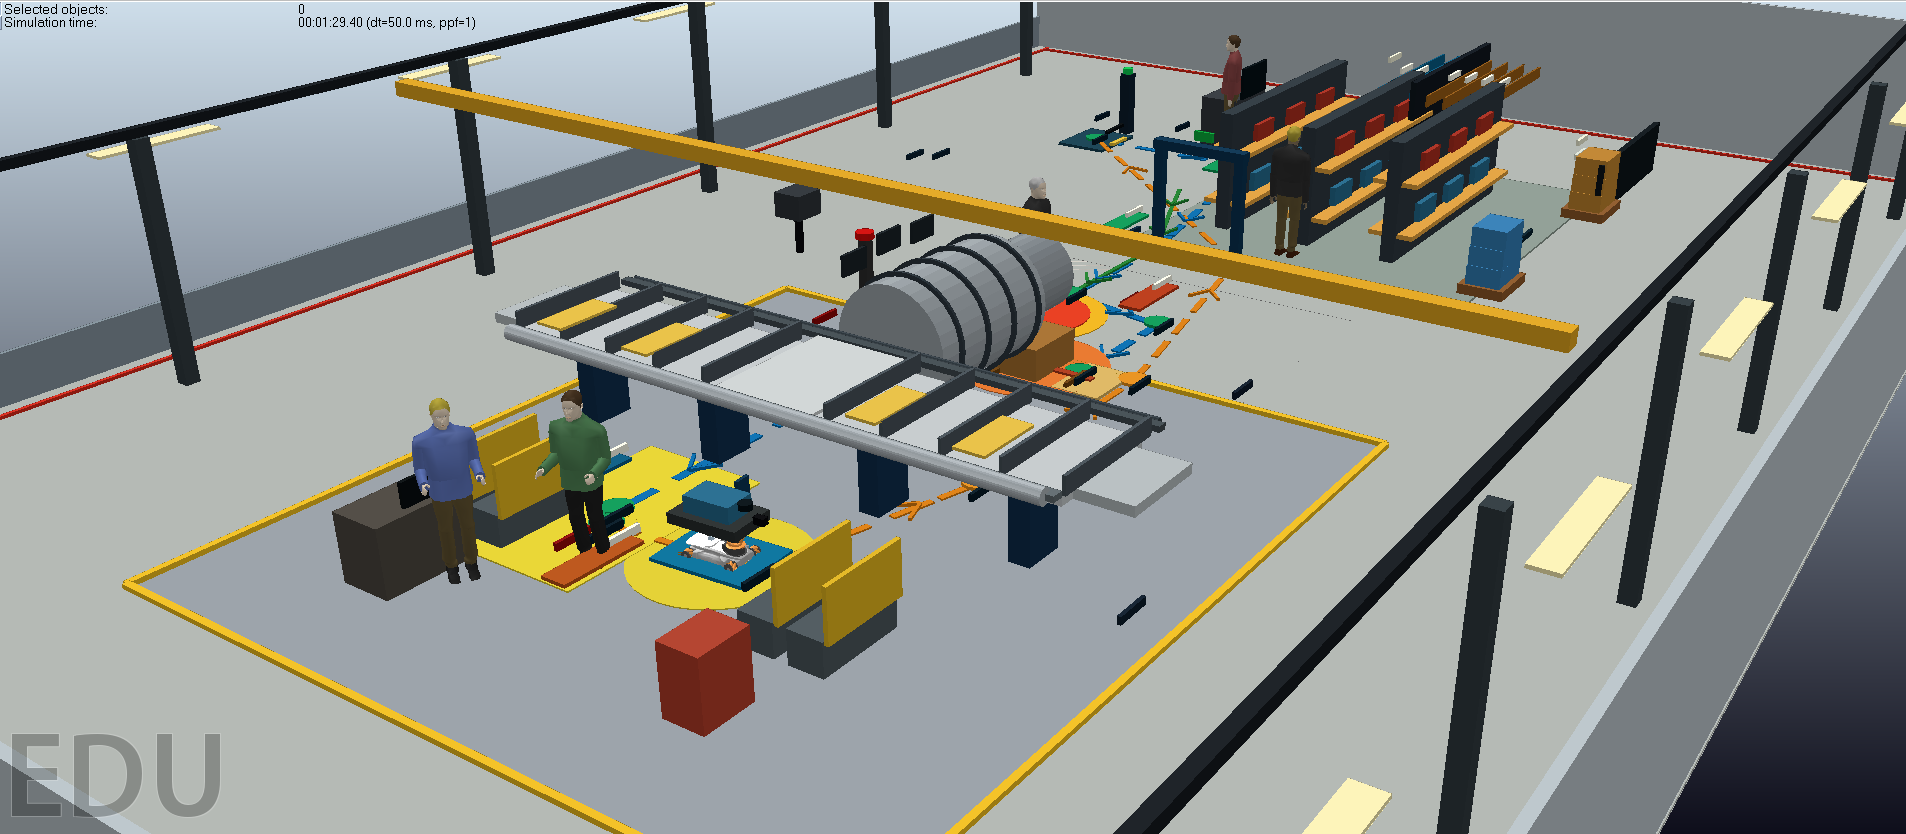
\includegraphics[width=6.55cm]{../figures/coppeliasim/ss2.png}};
  \node[anchor=center] at (2.78,2.20) {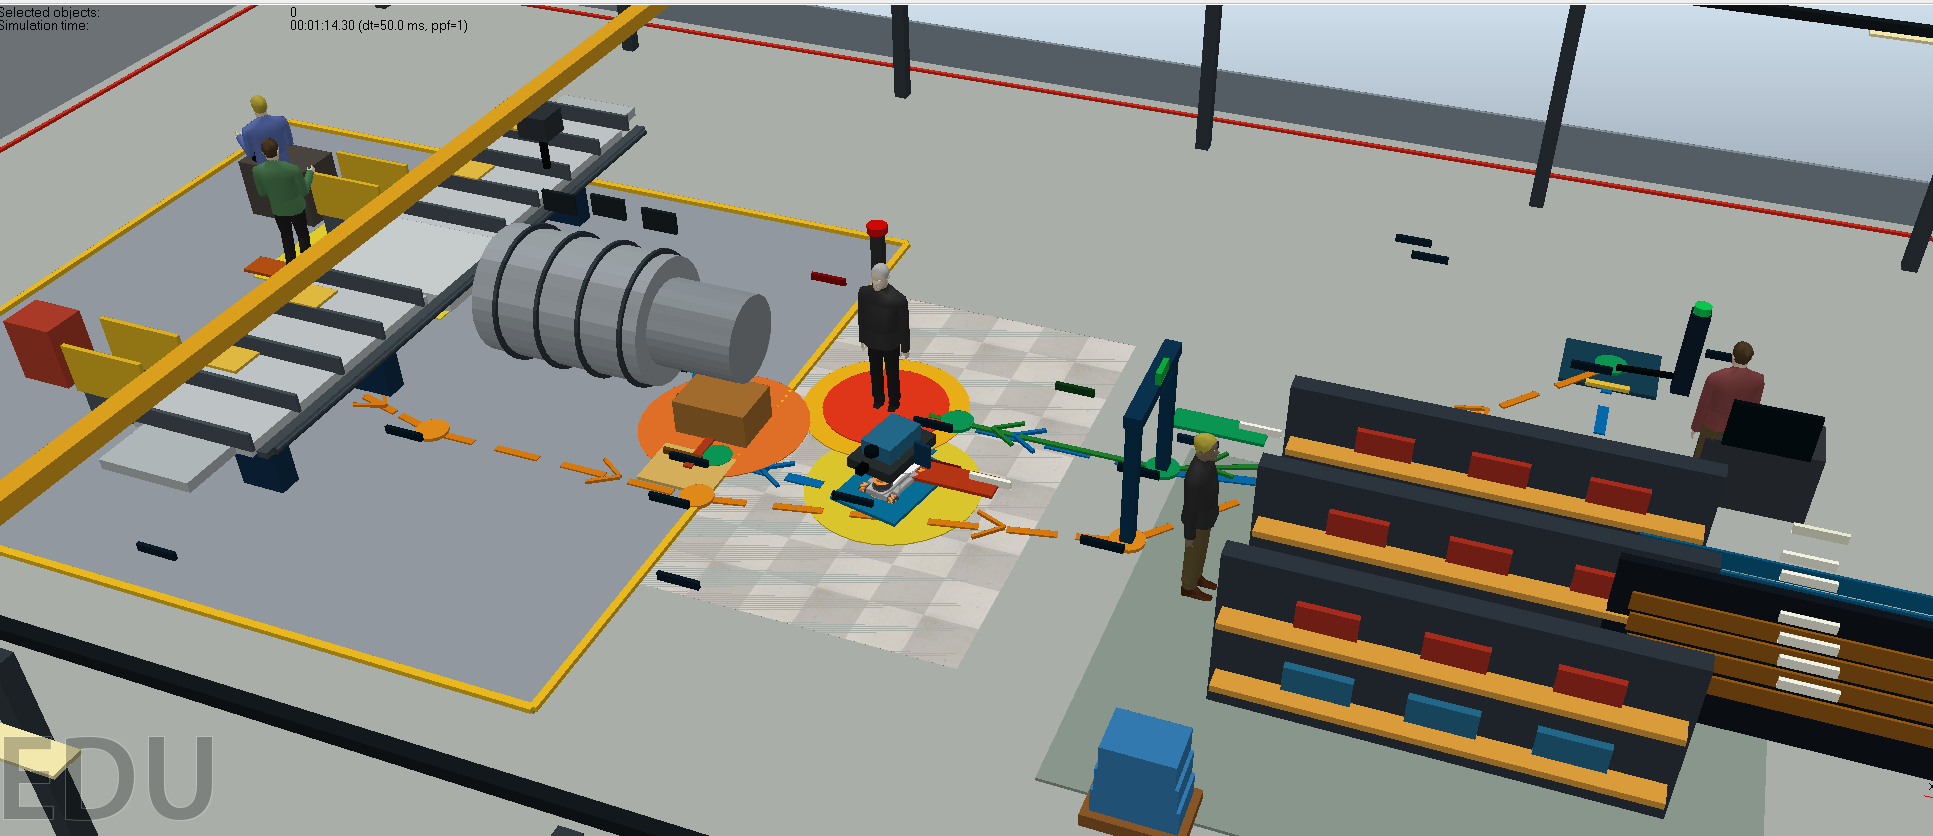
\includegraphics[width=3.08cm]{../figures/coppeliasim/ss1.png}};
  \node[anchor=center] at (6.16,2.20) {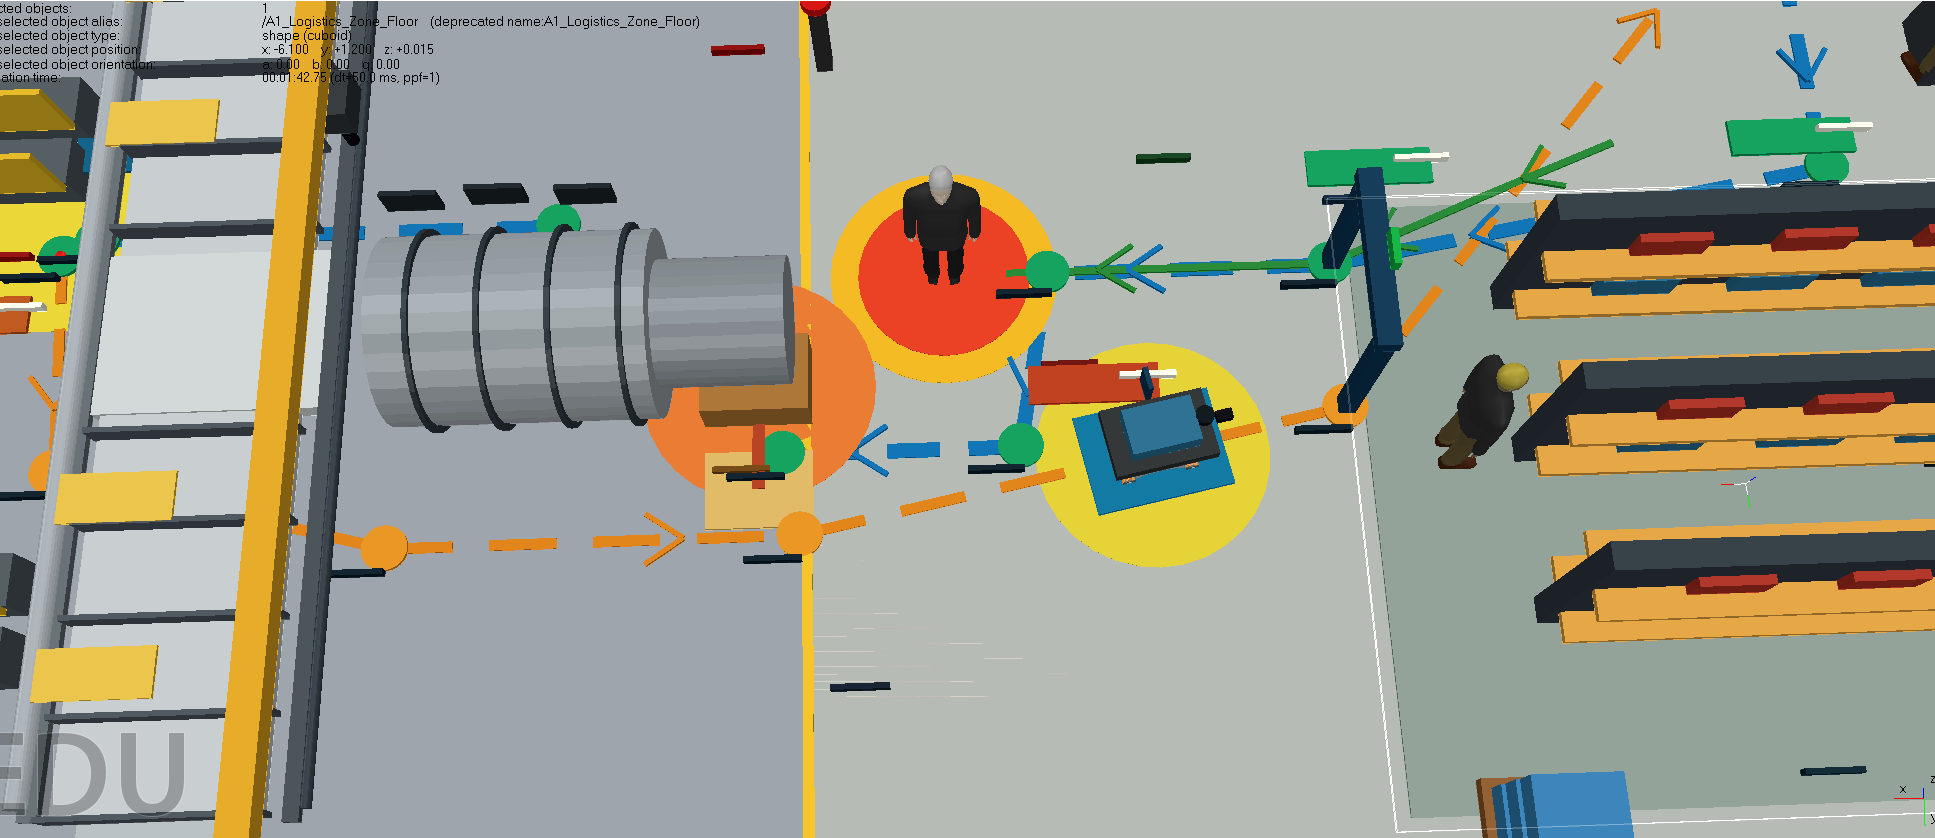
\includegraphics[width=3.08cm]{../figures/coppeliasim/ss3.png}};
  \node[anchor=west,font=\fontsize{15}{16}\selectfont\bfseries,text=Navy,text width=5.9cm] at (8.45,6.28) {Evidencia antes de planta};
  \signal{8.55}{5.22}{Escena real en CoppeliaSim: nave, HTP, kitting y operarios.}{Violet}
  \signal{8.55}{4.36}{YouBot como proxy mecanum; RB-KAIROS queda como referencia industrial.}{Teal}
  \signal{8.55}{3.50}{Ruta visible con parada/esquiva ante operario y zonas marcadas.}{Red}
  \signal{8.55}{2.64}{Tres capturas + \href{run:../coppeliasim/coppeliasim_demo.mp4}{v\'ideo \texttt{coppeliasim\_demo.mp4}} documentan la simulaci\'on.}{Amber}
  \node[anchor=west,font=\fontsize{6.35}{7.25}\selectfont,text=Muted,text width=5.25cm] at (8.55,1.42) {Criterios de salida: error \(\leq\!0{,}25\,\mathrm{m}\), cero contactos, rutas alternativas y reserva de bater\'ia. Licencia EDU visible; FAT/SAT valida carga real.};
\stopslide
\speakernote{Esta slide demuestra CoppeliaSim. No es un diagrama conceptual: son capturas reales de una escena con nave, HTP, kitting, operarios, ruta y punto FOD. YouBot valida la cinemática mecanum y la lógica de misión; RB-KAIROS queda como referencia industrial. CoppeliaSim valida rutas, paradas y flujo, pero FAT/SAT valida carga real y seguridad en planta.}

% 12
\startslide{Despliegue}{Tres fases con entregables y criterio de paso}{Green}
  \node[anchor=west,font=\fontsize{6.2}{7.0}\selectfont\bfseries,text=Green] at (1.00,6.60) {PLAN DE ESCALADO CON HITOS DE PASO};
  \draw[Line,line width=1.0pt] (1.40,4.64) -- (13.82,4.64);
  \foreach \x/\num/\ttl/\capex/\txt/\col in {
    2.10/1/{PILOTO\\S1--S12}/{237.444 \texteuro{}}/{Validar rutas, seguridad, registro y aceptaci\'on.}/Teal,
    7.30/7/{EXPANSI\'ON\\M4--M12}/{1.100.252 \texteuro{}}/{Cubrir l\'inea HTP si el piloto cumple criterios.}/Amber,
    12.50/17/{TENTATIVO\\A\~NO 2}/{2.495.768 \texteuro{}}/{Multi-zona, doble turno o crecimiento validado.}/Green}{
    \fill[\col!10,rounded corners=5pt] (\x-1.48,2.42) rectangle ++(2.96,2.64);
    \draw[\col,line width=0.55pt,rounded corners=5pt] (\x-1.48,2.42) rectangle ++(2.96,2.64);
    \node[anchor=west,font=\fontsize{22}{23}\selectfont\bfseries,text=\col] at (\x-1.18,4.54) {\num};
    \node[anchor=west,font=\fontsize{6.35}{7.0}\selectfont\bfseries,text=Ink,text width=1.58cm,align=left] at (\x-0.25,4.70) {\ttl};
    \node[anchor=west,font=\fontsize{6.3}{7.1}\selectfont\bfseries,text=\col] at (\x-1.18,3.96) {\capex};
    \node[anchor=north west,font=\fontsize{5.75}{6.5}\selectfont,text=Ink,text width=2.35cm,align=left] at (\x-1.18,3.45) {\txt};
  }

  \foreach \x/\label/\txt in {
    4.68/{Hito 1}/{KPIs piloto},
    9.88/{Hito 2}/{beneficio + flujo}}{
    \fill[white] (\x-0.38,4.20) rectangle ++(0.76,0.86);
    \draw[Red,line width=0.55pt,rounded corners=3pt] (\x-0.38,4.20) rectangle ++(0.76,0.86);
    \node[font=\fontsize{8.0}{8.6}\selectfont\bfseries,text=Red] at (\x,4.64) {\(\triangleright\)};
    \node[anchor=south,font=\fontsize{5.5}{6.2}\selectfont\bfseries,text=Ink,align=center,text width=2.25cm] at (\x,5.58) {\label};
    \node[anchor=north,font=\fontsize{5.0}{5.7}\selectfont,text=Muted,align=center,text width=2.25cm] at (\x,5.52) {\txt};
  }

  \draw[Teal,arrow,line width=0.85pt] (3.62,4.64) -- (4.20,4.64);
  \draw[Amber,arrow,line width=0.85pt] (8.82,4.64) -- (9.40,4.64);
  \draw[Green,arrow,line width=0.85pt] (13.92,4.64) -- (14.45,4.64);
  \fill[Green!8,rounded corners=5pt] (1.00,0.88) rectangle (13.86,1.78);
  \draw[Green!40,line width=0.45pt,rounded corners=5pt] (1.00,0.88) rectangle (13.86,1.78);
  \node[anchor=west,font=\fontsize{6.05}{6.95}\selectfont\bfseries,text=Navy,text width=11.95cm] at (1.22,1.48) {Criterio 1: misiones \(\geq 95\%\), registro \(\geq 98\%\), disponibilidad \(\geq 90\%\) y 0 contactos no previstos.};
  \node[anchor=west,font=\fontsize{5.85}{6.65}\selectfont\bfseries,text=Muted,text width=11.80cm] at (1.22,1.12) {Criterio 2: \(\geq 1{,}1\) HTP/mes de capacidad protegida o reducci\'on \(\geq 20\%\) de microesperas medidas.};
\stopslide
\speakernote{El despliegue se organiza por gates. Primero, 1 robot durante el piloto S1--S12 para validar rutas, seguridad, registro y aceptación. Luego, 7 robots solo si cumple KPIs y beneficio de flujo. Los 17 robots son tentativos: sirven para multi-zona, doble turno o reserva, no son una compra comprometida desde el inicio.}

% 13
\startslide{Presupuesto}{CAPEX y TCO por escenario}{Amber}
  \node[anchor=west,font=\fontsize{6.2}{7.1}\selectfont\bfseries,text=Muted] at (1.00,6.74) {CAPEX ESTIMADO SIN IVA};
  \node[anchor=west,font=\fontsize{14.2}{15.2}\selectfont\bfseries,text=Teal] at (1.00,6.22) {237.444 \texteuro{}};
  \node[anchor=west,font=\fontsize{14.2}{15.2}\selectfont\bfseries,text=Amber] at (5.30,6.22) {1.100.252 \texteuro{}};
  \node[anchor=west,font=\fontsize{14.2}{15.2}\selectfont\bfseries,text=Green] at (9.55,6.22) {2.495.768 \texteuro{}};
  \node[anchor=west,font=\fontsize{6.1}{6.9}\selectfont\bfseries,text=Muted] at (1.03,5.73) {1 ROBOT};
  \node[anchor=west,font=\fontsize{6.1}{6.9}\selectfont\bfseries,text=Muted] at (5.33,5.73) {7 ROBOTS};
  \node[anchor=west,font=\fontsize{6.1}{6.9}\selectfont\bfseries,text=Muted] at (9.58,5.73) {17 ROBOTS};

  \fill[Panel] (0.95,1.28) rectangle (14.05,5.32);
  \draw[Line,line width=0.45pt] (0.95,5.32) rectangle (14.05,1.28);
  \fill[Amber!18] (0.95,4.88) rectangle (14.05,5.32);
  \node[anchor=west,font=\fontsize{5.8}{6.5}\selectfont\bfseries,text=Ink] at (1.15,5.05) {Partida};
  \node[anchor=east,font=\fontsize{5.8}{6.5}\selectfont\bfseries,text=Ink] at (7.20,5.05) {1 robot};
  \node[anchor=east,font=\fontsize{5.8}{6.5}\selectfont\bfseries,text=Ink] at (10.55,5.05) {7 robots};
  \node[anchor=east,font=\fontsize{5.8}{6.5}\selectfont\bfseries,text=Ink] at (13.70,5.05) {17 robots*};

  \foreach \y/\part/\one/\seven/\seventeen/\col in {
    4.58/{Equipos: AMR + sensores + carga}/78.500/549.500/1.334.500/Teal,
    4.24/{Equipos: software flota + registro}/24.000/65.000/120.000/Violet,
    3.90/{Personal: ingeniería + simulación + CE}/46.000/126.000/245.000/Cyan,
    3.56/{Personal: instalación + SAT}/20.000/60.000/135.000/Green,
    3.22/{Personal: formación y cambio}/9.500/27.000/46.000/Amber,
    2.88/{Personal/OPEX: mantenimiento año 1}/6.300/44.100/106.800/Teal,
    2.54/{Logística: desplazamientos y medios}/5.000/20.000/40.000/Violet,
    2.20/{Materiales/docs: ciberseg. + aceptación}/7.000/18.000/36.000/Cyan,
    1.86/{Contingencia técnica 8\%}/15.704/72.768/165.064/Red,
    1.52/{Margen comercial 12\%}/25.440/117.884/267.404/Amber} {
    \fill[\col!9] (0.95,\y-0.15) rectangle (14.05,\y+0.17);
    \fill[\col] (1.12,\y-0.03) circle (0.055);
    \node[anchor=west,font=\fontsize{5.55}{6.25}\selectfont\bfseries,text=Ink] at (1.32,\y) {\part};
    \node[anchor=east,font=\fontsize{5.55}{6.25}\selectfont,text=Ink] at (7.20,\y) {\one};
    \node[anchor=east,font=\fontsize{5.55}{6.25}\selectfont,text=Ink] at (10.55,\y) {\seven};
    \node[anchor=east,font=\fontsize{5.55}{6.25}\selectfont,text=Ink] at (13.70,\y) {\seventeen};
  }
  \foreach \y in {3.73,2.71,1.69}{\draw[Ink,opacity=0.16,line width=0.45pt] (0.95,\y) -- (14.05,\y);}
  \node[anchor=west,font=\fontsize{5.55}{6.30}\selectfont\bfseries,text=Navy,text width=12.80cm] at (1.00,0.90) {Mapa r\'ubrica: personal, materiales, equipos y desplazamientos/log\'istica quedan etiquetados en la tabla.};
  \node[anchor=west,font=\fontsize{4.85}{5.50}\selectfont,text=Muted,text width=12.80cm] at (1.00,0.55) {TCO 3 a\~nos = CAPEX + soporte, licencias y mantenimiento recurrente: 284.044 \texteuro{} / 1.299.452 \texteuro{} / 2.951.368 \texteuro{}. *17 robots: aspiracional no comprometido.};
\stopslide
\speakernote{El presupuesto se presenta sin caja negra. Arriba están los tres CAPEX: 237.444 euros para piloto, 1,10 millones para 7 robots y 2,50 millones para 17. La tabla baja a partidas de equipos, software, personal, materiales, logística, contingencia y margen. También mapea literalmente las categorías del brief: personal, materiales, equipos y desplazamientos/logística.}

% 14
\startslide{ROI}{Decisi\'on por datos de piloto}{Teal}
  \roundbox{0.95}{1.35}{4.25}{5.10}{Teal!8}{Teal!40}
  \node[anchor=north west,font=\fontsize{11.2}{12.4}\selectfont\bfseries,text=Navy,text width=3.55cm,align=left] at (1.18,6.02) {Coste horario base};
  \node[anchor=west,font=\fontsize{6.05}{6.85}\selectfont,text=Ink] at (1.22,4.86) {Salario guía: 20.000--28.000 \texteuro{}/año.};
  \node[anchor=west,font=\fontsize{6.05}{6.85}\selectfont,text=Ink] at (1.22,4.52) {Caso central: 24.000 \texteuro{}.};
  \node[anchor=west,font=\fontsize{6.05}{6.85}\selectfont,text=Ink] at (1.22,4.18) {Coste empresa 1,35; 1.760 h/año.};
  \node[anchor=west,font=\fontsize{17.2}{18.2}\selectfont\bfseries,text=Teal] at (1.22,3.34) {18,4 \texteuro{}/h};
  \node[anchor=west,font=\fontsize{5.35}{6.05}\selectfont\bfseries,text=Navy,text width=3.70cm,align=left] at (1.25,2.82) {CHC = 24.000 \(\times\) 1,35 / 1.760\\= 18,4 \texteuro{}/h};
  \node[anchor=west,font=\fontsize{5.22}{5.95}\selectfont,text=Muted,text width=3.62cm] at (1.25,2.20) {No se asume sustituci\'on 1:1; se monetiza tiempo recuperado y continuidad de flujo.};
  \node[anchor=west,font=\fontsize{5.75}{6.55}\selectfont\bfseries,text=Red,text width=3.60cm] at (1.25,1.44) {El c\'alculo separa horas recuperadas, capacidad protegida e incidencias evitadas.};

  \node[anchor=west,font=\fontsize{6.1}{7.0}\selectfont\bfseries,text=Muted] at (5.70,6.40) {OPCI\'ON REAL DE ESCALADO};
  \fill[Teal!12] (5.70,5.82) rectangle (14.55,6.14);
  \node[anchor=west,font=\fontsize{5.8}{6.5}\selectfont\bfseries,text=Ink] at (5.92,5.98) {Fase};
  \node[anchor=west,font=\fontsize{5.8}{6.5}\selectfont\bfseries,text=Ink] at (7.70,5.98) {Inversi\'on};
  \node[anchor=west,font=\fontsize{5.8}{6.5}\selectfont\bfseries,text=Ink] at (9.55,5.98) {Informaci\'on que compra};
  \foreach \y/\fase/\inv/\info/\col in {
    5.28/{Piloto}/{237 k\texteuro{}}/{seguridad, aceptaci\'on, rutas y KPIs reales}/Teal,
    4.36/{7 robots}/{1,10 M\texteuro{}}/{s\'olo si demuestra \(\geq 1{,}25\) HTP/mes protegido}/Amber,
    3.44/{17 robots}/{2,50 M\texteuro{}}/{decisi\'on estrat\'egica: multi-zona o doble turno}/Green}{
    \draw[Line,line width=0.35pt] (5.70,\y-0.36) -- (14.55,\y-0.36);
    \node[anchor=west,font=\fontsize{6.5}{7.4}\selectfont\bfseries,text=\col] at (5.92,\y) {\fase};
    \node[anchor=west,font=\fontsize{6.2}{7.0}\selectfont\bfseries,text=Ink] at (7.70,\y) {\inv};
    \node[anchor=west,font=\fontsize{6.05}{6.85}\selectfont,text=Ink,text width=4.85cm] at (9.55,\y) {\info};
  }

  \fill[Amber!10,rounded corners=5pt] (5.70,0.94) rectangle (13.82,2.54);
  \draw[Amber!50,line width=0.45pt,rounded corners=5pt] (5.70,0.94) rectangle (13.82,2.54);
  \node[anchor=west,font=\fontsize{6.05}{6.95}\selectfont\bfseries,text=Amber] at (5.92,2.24) {Umbral econ\'omico defendible};
  \node[anchor=west,font=\fontsize{5.55}{6.35}\selectfont\bfseries,text=Navy,text width=7.30cm] at (5.92,1.82) {Condici\'on para 7 robots: \(\geq 1{,}1\) HTP/mes de capacidad protegida con margen interno estimado de 20.000 \texteuro{}/HTP.};
  \node[anchor=west,font=\fontsize{5.15}{5.9}\selectfont,text=Muted,text width=7.30cm] at (5.92,1.16) {No es precio p\'ublico ni venta de pieza: es valor econ\'omico interno del caso central; sensibilidad 10/20/50 k\texteuro{} en el informe.};
\stopslide
\speakernote{En ROI no vendo humo. El coste horario base es 18,4 euros por hora, pero la propuesta no asume sustitución uno a uno de operarios. El piloto compra información: seguridad, aceptación, rutas y KPIs reales. Para pasar a 7 robots se necesita demostrar al menos 1,25 HTP al mes de capacidad protegida con un margen interno estimado de 20.000 euros por HTP, o un beneficio equivalente medido.}

% 15
\startslide{Oferta comercial}{Entregables y condiciones de aceptaci\'on}{Amber}
  \node[anchor=west,font=\fontsize{13.5}{14.7}\selectfont\bfseries,text=Navy] at (0.95,6.48) {Entregables de la fase piloto};
  \foreach \y/\ttl/\txt/\col in {
    5.70/{Mapa operativo}/{rutas permitidas, zonas lentas, puntos de carga y entrega}/Teal,
    5.03/{Configuraci\'on AMR}/{misiones, prioridades, retorno de \'utiles y reglas de bater\'ia}/Green,
    4.36/{Registro}/{BD de misiones, RFID--QR, HMI y excepciones}/Violet,
    3.69/{FOD preventivo}/{rondas con imagen, evento y revisi\'on humana}/Red,
    3.02/{Validaci\'on CoppeliaSim}/{pruebas de SLAM, ruta bloqueada, TEB y misi\'on FOD}/Cyan,
    2.35/{Criterio de escalado}/{informe de KPIs, beneficio medido y decisi\'on 1 \(\rightarrow\) 7}/Amber} {
    \fill[\col] (1.02,\y+0.03) circle (0.055);
    \node[anchor=west,font=\fontsize{6.8}{7.7}\selectfont\bfseries,text=\col] at (1.24,\y+0.10) {\ttl};
    \node[anchor=west,font=\fontsize{5.75}{6.55}\selectfont,text=Ink,text width=6.05cm] at (1.24,\y-0.22) {\txt};
  }

  \roundbox{8.62}{1.78}{5.23}{4.75}{Amber!8}{Amber!45}
  \node[anchor=west,font=\fontsize{6.2}{7.0}\selectfont\bfseries,text=Muted] at (8.92,6.12) {CRITERIOS DE ACEPTACI\'ON};
  \foreach \y/\crit/\umbral/\col in {
    5.48/{Seguridad}/{0 contactos no previstos y 0 incidentes con da\~no}/Red,
    4.82/{Misiones}/{\(\geq 95\%\) completadas}/Teal,
    4.16/{Registro}/{\(\geq 98\%\) completo}/Violet,
    3.50/{Disponibilidad}/{\(\geq 90\%\) en turno piloto}/Green,
    2.84/{FOD}/{eventos con evidencia revisable}/Amber,
    2.18/{Usuarios}/{formaci\'on y protocolo de parada entendidos}/Cyan} {
    \draw[\col,line width=0.55pt] (8.92,\y-0.25) -- (13.45,\y-0.25);
    \node[anchor=west,font=\fontsize{6.25}{7.2}\selectfont\bfseries,text=\col] at (8.98,\y) {\crit};
    \node[anchor=west,font=\fontsize{5.75}{6.65}\selectfont,text=Ink,text width=2.35cm] at (10.78,\y) {\umbral};
  }
  \node[anchor=west,font=\fontsize{5.65}{6.4}\selectfont\bfseries,text=Red] at (8.92,1.32) {Pago por hitos};
  \foreach \x/\hito/\pago in {
    8.92/{M0 Inicio}/{30\%},
    10.10/{M3 Entrega}/{40\%},
    11.38/{M5 Valid.}/{20\%},
    12.66/{M6 Cierre}/{10\%}}{
    \fill[Red!6,rounded corners=2pt] (\x,0.78) rectangle ++(1.15,0.38);
    \draw[Red!40,line width=0.25pt,rounded corners=2pt] (\x,0.78) rectangle ++(1.15,0.38);
    \node[anchor=west,font=\fontsize{4.75}{5.3}\selectfont\bfseries,text=Ink] at (\x+0.07,1.02) {\hito};
    \node[anchor=west,font=\fontsize{5.25}{5.9}\selectfont\bfseries,text=Red] at (\x+0.07,0.86) {\pago};
  }
\stopslide
\speakernote{La oferta comercial separa entregables, criterios y pagos. En entregables: mapa operativo, configuración AMR, registro, FOD preventivo, validación CoppeliaSim y criterio de escalado. En aceptación: seguridad, misiones, registro, disponibilidad, FOD y usuarios formados. El pago por hitos evita pagar toda la fase sin validar entrega y KPIs.}

% 16
\startslide{Recomendación}{Medir antes de escalar}{Green}
  \node[anchor=west,font=\fontsize{25}{26}\selectfont\bfseries,text=Green] at (0.95,6.22) {1 robot primero};
  \node[anchor=west,font=\fontsize{9.0}{10.4}\selectfont,text=Ink,text width=6.15cm] at (1.02,5.20) {Validar rutas, seguridad, entregas, registro, FOD y aceptaci\'on operativa. Escalar s\'olo con datos.};

  \node[anchor=west,font=\fontsize{7.0}{8.0}\selectfont\bfseries,text=Muted] at (1.05,3.98) {PLAN DE 12 SEMANAS · PILOTO};
  \draw[Line,line width=0.75pt] (1.05,3.36) -- (14.45,3.36);
  \foreach \x/\w/\ttl/\sub/\col in {
    1.05/2.05/{S1}/{levantamiento de planta}/Teal,
    3.45/3.65/{S2--S4}/{mapa, rutas, carga y SAT inicial}/Amber,
    7.45/3.65/{S5--S10}/{operaci\'on piloto y captura de KPIs}/Green,
    11.45/1.35/{S11}/{revisi\'on KPI}/Violet,
    13.10/1.35/{S12}/{Decisi\'on 1}/Red}{
    \fill[\col!11,rounded corners=4pt] (\x,2.70) rectangle ++(\w,0.76);
    \draw[\col,line width=0.45pt,rounded corners=4pt] (\x,2.70) rectangle ++(\w,0.76);
    \node[anchor=west,font=\fontsize{7.0}{7.8}\selectfont\bfseries,text=\col] at (\x+0.15,3.18) {\ttl};
    \node[anchor=west,font=\fontsize{5.35}{6.05}\selectfont,text=Ink,text width=\w cm] at (\x+0.15,2.90) {\sub};
  }

  \draw[Line,line width=0.6pt] (1.05,2.20) -- (14.85,2.20);
  \foreach \x/\num/\txt/\col in {
    1.05/{1}/{Confirmar zona piloto, puntos de carga/entrega y restricciones de seguridad.}/Teal,
    5.35/{2}/{Ejecutar misiones kitting/FOD con registro RFID/QR y eventos revisables.}/Amber,
    9.85/{3}/{Decidir escalado con KPIs, umbral econ\'omico y aceptaci\'on de usuarios.}/Green}{
    \fill[\col] (\x,1.50) circle (0.16);
    \node[font=\fontsize{6.4}{7.0}\selectfont\bfseries,text=white] at (\x,1.50) {\num};
    \node[anchor=west,font=\fontsize{6.25}{7.15}\selectfont\bfseries,text=Navy,text width=3.45cm] at (\x+0.28,1.50) {\txt};
  }
  \node[anchor=west,font=\fontsize{5.8}{6.6}\selectfont,text=Muted] at (1.05,0.72) {Semanas = piloto; meses = expansi\'on posterior. Lunabotics \textbullet{} contacto@lunabotics.aero \textbullet{} Actividad 1 MROB-VIU 2026};
\stopslide
\speakernote{La recomendación final es deliberadamente conservadora: un robot primero. En doce semanas se levanta planta, se configuran rutas, se opera el piloto y se revisan KPIs. La decisión comercial llega al final, no al principio. Si no hay datos de seguridad, aceptación y beneficio, Lunabotics no recomienda escalar.}

% 22
\startslide{AMDEC piloto}{Riesgos principales y mitigaciones}{Teal}
  \node[anchor=west,font=\fontsize{7.7}{8.8}\selectfont\bfseries,text=Navy,text width=13.00cm] at (1.00,6.42) {La propuesta no oculta incertidumbres: las punt\'ua y reduce antes de escalar a flota. RPN = Severidad \(\times\) Ocurrencia \(\times\) Detecci\'on.};

  \fill[Teal!12] (0.95,5.62) rectangle (14.75,5.96);
  \node[anchor=west,font=\fontsize{5.75}{6.4}\selectfont\bfseries,text=Ink] at (1.12,5.78) {Modo de fallo};
  \node[anchor=west,font=\fontsize{5.75}{6.4}\selectfont\bfseries,text=Ink] at (5.82,5.78) {Mitigaci\'on};
  \node[font=\fontsize{5.75}{6.4}\selectfont\bfseries,text=Ink] at (10.32,5.78) {S};
  \node[font=\fontsize{5.75}{6.4}\selectfont\bfseries,text=Ink] at (11.00,5.78) {O};
  \node[font=\fontsize{5.75}{6.4}\selectfont\bfseries,text=Ink] at (11.68,5.78) {D};
  \node[font=\fontsize{5.75}{6.4}\selectfont\bfseries,text=Ink] at (12.55,5.78) {RPN};
  \node[anchor=west,font=\fontsize{5.75}{6.4}\selectfont\bfseries,text=Ink] at (13.10,5.78) {Salida};
  \foreach \y/\fail/\mit/\s/\o/\d/\rpn/\out/\col in {
    5.20/{Contacto con operario}/{zonas lentas, esc\'aner, bumper y E-stop}/9/2/2/36/{SAT}/Red,
    4.58/{FOD generado por AMR}/{portakits cerrados, limpieza y ronda RGB-D}/8/3/3/72/{QA}/Amber,
    3.96/{Pasillo bloqueado / gr\'ua puente}/{zonificaci\'on din\'amica y replanificaci\'on TEB}/7/4/3/84/{Mapa}/Green,
    3.34/{P\'erdida RFID/QR}/{doble lectura, HMI y cierre manual controlado}/6/3/3/54/{Registro}/Violet,
    2.72/{WiFi / BD no disponible}/{buffer local y procedimiento manual de contingencia}/5/3/4/60/{Fallback}/Cyan,
    2.10/{Escalado prematuro}/{Criterios 1 y 2 con umbral econ\'omico medido}/8/2/2/32/{Direcci\'on}/Teal}{
    \fill[\col!7] (0.95,\y-0.21) rectangle (14.75,\y+0.23);
    \draw[Line,line width=0.25pt] (0.95,\y-0.21) -- (14.75,\y-0.21);
    \node[anchor=west,font=\fontsize{5.65}{6.35}\selectfont\bfseries,text=\col,text width=4.35cm] at (1.12,\y+0.02) {\fail};
    \node[anchor=west,font=\fontsize{5.45}{6.15}\selectfont,text=Ink,text width=4.25cm] at (5.82,\y+0.02) {\mit};
    \node[font=\fontsize{5.85}{6.45}\selectfont\bfseries,text=Ink] at (10.32,\y+0.02) {\s};
    \node[font=\fontsize{5.85}{6.45}\selectfont\bfseries,text=Ink] at (11.00,\y+0.02) {\o};
    \node[font=\fontsize{5.85}{6.45}\selectfont\bfseries,text=Ink] at (11.68,\y+0.02) {\d};
    \node[font=\fontsize{5.85}{6.45}\selectfont\bfseries,text=\col] at (12.55,\y+0.02) {\rpn};
    \node[anchor=west,font=\fontsize{5.3}{6.0}\selectfont\bfseries,text=Muted] at (13.10,\y+0.02) {\out};
  }

  \node[anchor=west,font=\fontsize{5.85}{6.65}\selectfont\bfseries,text=Navy,text width=12.90cm] at (1.05,1.18) {Riesgos aeron\'auticos expl\'icitos: AS9100/NAS 412, FOD del propio AMR y coexistencia con gr\'ua puente. S/O/D usa una escala AMDEC simplificada para priorizar el piloto.};
\stopslide
\speakernote{El AMDEC muestra que la propuesta reconoce riesgos. Los más importantes son contacto con operario, FOD generado por el propio AMR, pasillo bloqueado o grúa puente, pérdida RFID/QR, caída de WiFi y escalado prematuro. Cada riesgo tiene mitigación y una salida de control. La tabla prioriza la incertidumbre antes del piloto.}

% 23
\ifnum\value{slide}>0\clearpage\fi
\stepcounter{slide}%
\begin{tikzpicture}[remember picture,overlay,x=1cm,y=1cm]
\begin{scope}[shift={(current page.south west)}]
  \fill[Paper] (0,0) rectangle (16,9);
  \node[font=\fontsize{34}{36}\selectfont\bfseries,text=Navy] at (8,4.80) {¡Muchas gracias!};
\end{scope}
\end{tikzpicture}
\speakernote{Cerrar sin explicar de más. Mantener contacto visual, dar las gracias y dejar espacio para preguntas del profesor.}

% 24
\startslide{}{Referencias}{Violet}
  \node[anchor=west,font=\fontsize{7.3}{8.2}\selectfont\bfseries,text=Navy,text width=12.9cm] at (1.00,6.54) {Selecci\'on de referencias usadas en el informe t\'ecnico y citadas en la oferta.};

  \draw[Line,line width=0.45pt] (1.00,6.10) -- (14.45,6.10);
  \foreach \x/\y/\num/\txt in {
    1.05/5.54/{[1]}/{ISO 3691-4, \textit{Driverless industrial trucks and their systems}, seguridad AMR/AGV.},
    1.05/4.80/{[2]}/{SAE NAS 412, \textit{Foreign Object Damage / Foreign Object Debris Prevention}.},
    1.05/4.06/{[3]}/{EN 9100 / AS9100D, sistemas de gesti\'on de calidad aeroespacial.},
    1.05/3.32/{[4]}/{Coppelia Robotics, \textit{CoppeliaSim User Manual}, documentaci\'on del simulador, 2026.},
    8.05/5.54/{[5]}/{Siegwart, Nourbakhsh y Scaramuzza, \textit{Introduction to Autonomous Mobile Robots}, MIT Press, 2011.},
    8.05/4.80/{[6]}/{Robotnik Automation, \textit{RB-KAIROS Datasheet} y p\'agina de producto, 2024--2026.},
    8.05/4.06/{[7]}/{AGILOX Services GmbH, \textit{AGILOX ODM}; MiR, \textit{MiR250 Specifications}, benchmarks AMR.},
    8.05/3.32/{[8]}/{Intel RealSense D435i, Hokuyo UST-10LX y Zebra FX9600, referencias de sensores.}}{
    \node[anchor=west,font=\fontsize{5.75}{6.45}\selectfont\bfseries,text=Muted] at (\x,\y) {\num};
    \node[anchor=west,font=\fontsize{5.35}{6.10}\selectfont,text=Ink,text width=5.72cm] at (\x+0.55,\y) {\txt};
  }
  \node[anchor=west,font=\fontsize{5.7}{6.5}\selectfont,text=Muted,text width=11.80cm] at (1.05,1.10) {Referencias completas, enlaces y fechas de consulta: bibliograf\'ia del informe t\'ecnico.};
\stopslide
\speakernote{Cierro con las referencias principales. No hace falta leerlas todas: sirven para demostrar que las normas, robots, sensores y simulador tienen soporte. Mencionaría cuatro familias si hay tiempo: seguridad AMR con ISO 3691-4, calidad aeronáutica con EN/AS9100, FOD con NAS 412 y simulación con CoppeliaSim. Las referencias completas están en la bibliografía del informe.}

\end{document}


